\documentclass[tikz,multi=tikzpicture,border=7pt]{standalone}
\usepackage{amsmath,amssymb}
\usetikzlibrary{arrows.meta,calc,positioning,decorations.pathreplacing}

% CBOW: persistent parameter tables, sample-dependent sparse connectivity.
% Compile using: pdflatex -interaction=nonstopmode -halt-on-error cbow_dynamic_connections.tex
\definecolor{ink}{HTML}{17243B}
\definecolor{muted}{HTML}{53647A}
\definecolor{panelbg}{HTML}{F7FAFE}
\definecolor{line}{HTML}{CBD5E1}
\definecolor{selectA}{HTML}{DFF5E9}
\definecolor{selectB}{HTML}{DDEBFF}
\definecolor{teal}{HTML}{15846A}
\definecolor{blue}{HTML}{336BC9}
\definecolor{violet}{HTML}{6A50A7}
\definecolor{pink}{HTML}{B33D5E}
\definecolor{paleviolet}{HTML}{EAE5F7}
\definecolor{palepink}{HTML}{FBE6EC}

\tikzset{
  >={Latex[length=2.7mm]},
  flow/.style={->,draw=ink,line width=1.1pt},
  linkA/.style={->,draw=teal,line width=1.35pt},
  linkB/.style={->,draw=blue,line width=1.35pt},
  reverse/.style={->,draw=pink,line width=1.3pt},
  box/.style={draw=line,fill=white,rounded corners=4pt,inner sep=5pt,align=center},
  avg/.style={draw=violet,fill=paleviolet,rounded corners=5pt,align=center,minimum width=2.0cm,minimum height=1.0cm},
  classifier/.style={draw=violet,fill=paleviolet,rounded corners=5pt,align=center,minimum width=2.4cm,minimum height=1.0cm},
  stage/.style={draw=line,fill=white,rounded corners=5pt,align=center,minimum width=2.3cm,minimum height=1.0cm},
  target/.style={draw=pink,fill=palepink,rounded corners=5pt,align=center,minimum width=2.6cm,minimum height=1.0cm},
}

\begin{document}
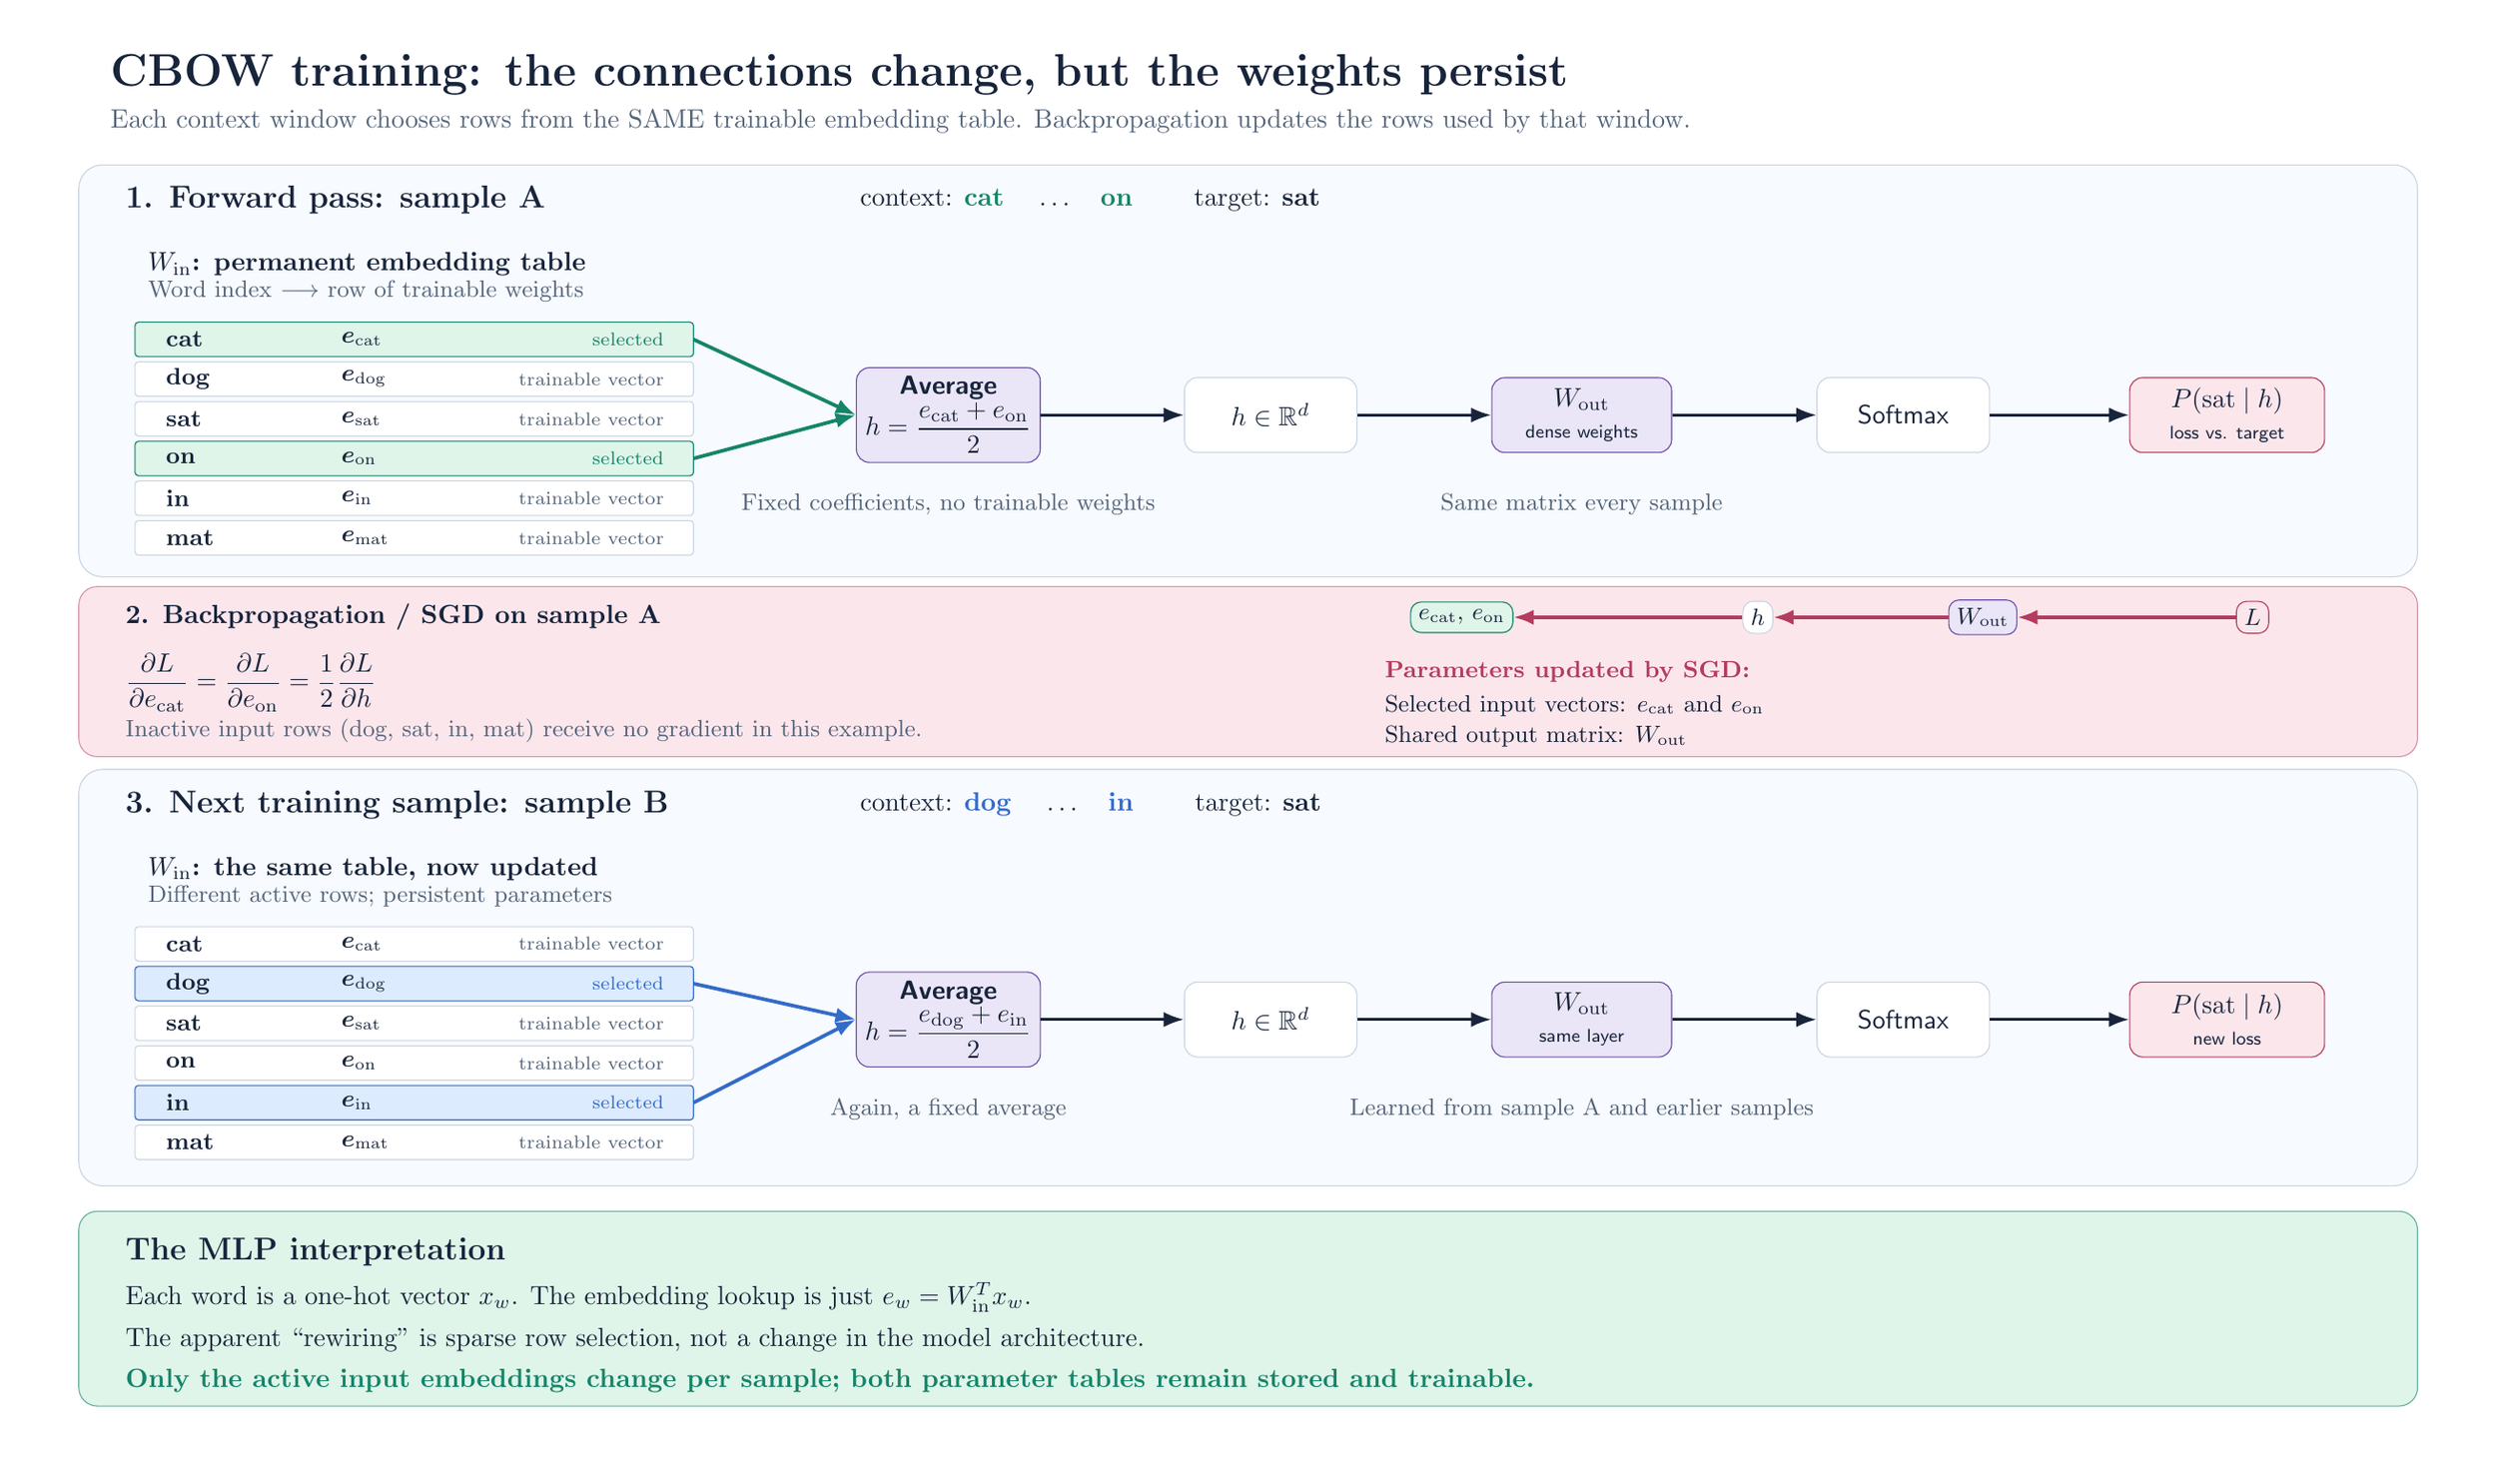
\begin{tikzpicture}[x=1cm,y=1cm,font=\sffamily,text=ink]

% Canvas = 32.6 x 19.1 cm. This standalone figure scales well in PDF.
\fill[white] (0,0) rectangle (32.6,19.1);
\node[anchor=west,font=\bfseries\LARGE] at (1,18.45)
  {CBOW training: the connections change, but the weights persist};
\node[anchor=west,text=muted,font=\normalsize] at (1,17.83)
  {Each context window chooses rows from the SAME trainable embedding table. Backpropagation updates the rows used by that window.};

% --- Panel A ---
\filldraw[fill=panelbg,draw=line,rounded corners=9pt] (0.7,11.75) rectangle (31.9,17.25);
\node[anchor=west,font=\bfseries\large] at (1.2,16.78) {1. Forward pass: sample A};
\node[anchor=west,font=\normalsize] at (11.0,16.78)
  {context: \textcolor{teal}{\textbf{cat}} \quad \ldots \quad \textcolor{teal}{\textbf{on}} \qquad target: \textbf{sat}};
\node[anchor=west,font=\bfseries\normalsize] at (1.5,15.92)
  {$W_{\mathrm{in}}$: permanent embedding table};
\node[anchor=west,text=muted,font=\small] at (1.5,15.56) {Word index $\longrightarrow$ row of trainable weights};

% Table A rows, equal row pitch 0.53 cm.
\foreach \word/\symbol/\y in {
  cat/cat/14.92,dog/dog/14.39,sat/sat/13.86,on/on/13.33,in/in/12.80,mat/mat/12.27}
{
  \filldraw[fill=white,draw=line,rounded corners=1.3pt] (1.45,\y-0.23) rectangle (8.90,\y+0.23);
  \node[anchor=west,font=\small\bfseries] at (1.74,\y) {\word};
  \node[anchor=west,font=\small] at (4.08,\y) {$\boldsymbol e_{\mathrm{\symbol}}$};
  \node[anchor=east,text=muted,font=\scriptsize] at (8.63,\y) {trainable vector};
}
\filldraw[fill=selectA,draw=teal,rounded corners=1.3pt] (1.45,14.69) rectangle (8.9,15.15);
\node[anchor=west,font=\small\bfseries] at (1.74,14.92) {cat};
\node[anchor=west,font=\small] at (4.08,14.92) {$\boldsymbol e_{\mathrm{cat}}$};
\node[anchor=east,font=\scriptsize,text=teal] at (8.63,14.92) {selected};
\filldraw[fill=selectA,draw=teal,rounded corners=1.3pt] (1.45,13.10) rectangle (8.9,13.56);
\node[anchor=west,font=\small\bfseries] at (1.74,13.33) {on};
\node[anchor=west,font=\small] at (4.08,13.33) {$\boldsymbol e_{\mathrm{on}}$};
\node[anchor=east,font=\scriptsize,text=teal] at (8.63,13.33) {selected};

\node[avg] (avgA) at (12.3,13.91) {\textbf{Average}\\$\displaystyle h=\frac{e_{\rm cat}+e_{\rm on}}{2}$};
\node[stage] (hA) at (16.6,13.91) {$h\in\mathbb{R}^d$};
\node[classifier] (outA) at (20.75,13.91) {$W_{\rm out}$\\\scriptsize dense weights};
\node[stage] (softA) at (25.04,13.91) {Softmax};
\node[target] (targetA) at (29.36,13.91) {$P(\mathrm{sat}\mid h)$\\\scriptsize loss vs. target};
\draw[linkA] (8.9,14.92) -- (avgA.west);
\draw[linkA] (8.9,13.33) -- (avgA.west);
\draw[flow] (avgA.east) -- (hA.west);
\draw[flow] (hA.east) -- (outA.west);
\draw[flow] (outA.east) -- (softA.west);
\draw[flow] (softA.east) -- (targetA.west);
\node[anchor=north,font=\small,text=muted] at (12.3,12.98) {Fixed coefficients, no trainable weights};
\node[anchor=north,font=\small,text=muted] at (20.75,12.98) {Same matrix every sample};

% --- Gradient strip: clear separation between path and equations ---
\filldraw[draw=pink!55,fill=palepink,rounded corners=7pt]
  (0.7,9.35) rectangle (31.9,11.62);
\node[anchor=west,font=\bfseries\normalsize] at (1.2,11.22)
  {2. Backpropagation / SGD on sample A};

% Reverse gradient path occupies the upper-right section only.
\node[box,draw=teal,fill=selectA,inner sep=3pt,font=\small] (gradEmb) at (19.15,11.21)
  {$e_{\rm cat},\,e_{\rm on}$};
\node[box,inner sep=3pt,font=\small] (gradH) at (23.10,11.21) {$h$};
\node[box,draw=violet,fill=paleviolet,inner sep=3pt,font=\small] (gradW) at (26.10,11.21)
  {$W_{\rm out}$};
\node[box,draw=pink,fill=palepink,inner sep=3pt,font=\small] (gradL) at (29.70,11.21) {$L$};
\draw[reverse] (gradL.west) -- (gradW.east);
\draw[reverse] (gradW.west) -- (gradH.east);
\draw[reverse] (gradH.west) -- (gradEmb.east);

% Explicitly separate mathematical derivation from the annotations.
\node[anchor=north west,font=\normalsize] at (1.2,10.85)
  {$\displaystyle \frac{\partial L}{\partial e_{\rm cat}}
                =\frac{\partial L}{\partial e_{\rm on}}
                =\frac{1}{2}\frac{\partial L}{\partial h}$};
\node[anchor=west,text=muted,font=\small] at (1.2,9.69)
  {Inactive input rows (dog, sat, in, mat) receive no gradient in this example.};

% A separated summary of the updates, to the right of the equation.
\node[anchor=west,font=\bfseries\small,text=pink] at (18.0,10.48)
  {Parameters updated by SGD:};
\node[anchor=west,font=\small] at (18.0,10.03)
  {Selected input vectors: $e_{\rm cat}$ and $e_{\rm on}$};
\node[anchor=west,font=\small] at (18.0,9.62)
  {Shared output matrix: $W_{\rm out}$};

% --- Panel B ---
\filldraw[fill=panelbg,draw=line,rounded corners=9pt] (0.7,3.62) rectangle (31.9,9.18);
\node[anchor=west,font=\bfseries\large] at (1.2,8.71) {3. Next training sample: sample B};
\node[anchor=west,font=\normalsize] at (11.0,8.71)
  {context: \textcolor{blue}{\textbf{dog}} \quad \ldots \quad \textcolor{blue}{\textbf{in}} \qquad target: \textbf{sat}};
\node[anchor=west,font=\bfseries\normalsize] at (1.5,7.85)
  {$W_{\mathrm{in}}$: the same table, now updated};
\node[anchor=west,text=muted,font=\small] at (1.5,7.49) {Different active rows; persistent parameters};

\foreach \word/\symbol/\y in {
  cat/cat/6.85,dog/dog/6.32,sat/sat/5.79,on/on/5.26,in/in/4.73,mat/mat/4.20}
{
  \filldraw[fill=white,draw=line,rounded corners=1.3pt] (1.45,\y-0.23) rectangle (8.90,\y+0.23);
  \node[anchor=west,font=\small\bfseries] at (1.74,\y) {\word};
  \node[anchor=west,font=\small] at (4.08,\y) {$\boldsymbol e_{\mathrm{\symbol}}$};
  \node[anchor=east,text=muted,font=\scriptsize] at (8.63,\y) {trainable vector};
}
\filldraw[fill=selectB,draw=blue,rounded corners=1.3pt] (1.45,6.09) rectangle (8.9,6.55);
\node[anchor=west,font=\small\bfseries] at (1.74,6.32) {dog};
\node[anchor=west,font=\small] at (4.08,6.32) {$\boldsymbol e_{\mathrm{dog}}$};
\node[anchor=east,font=\scriptsize,text=blue] at (8.63,6.32) {selected};
\filldraw[fill=selectB,draw=blue,rounded corners=1.3pt] (1.45,4.50) rectangle (8.9,4.96);
\node[anchor=west,font=\small\bfseries] at (1.74,4.73) {in};
\node[anchor=west,font=\small] at (4.08,4.73) {$\boldsymbol e_{\mathrm{in}}$};
\node[anchor=east,font=\scriptsize,text=blue] at (8.63,4.73) {selected};

\node[avg] (avgB) at (12.3,5.84) {\textbf{Average}\\$\displaystyle h=\frac{e_{\rm dog}+e_{\rm in}}{2}$};
\node[stage] (hB) at (16.6,5.84) {$h\in\mathbb{R}^d$};
\node[classifier] (outB) at (20.75,5.84) {$W_{\rm out}$\\\scriptsize same layer};
\node[stage] (softB) at (25.04,5.84) {Softmax};
\node[target] (targetB) at (29.36,5.84) {$P(\mathrm{sat}\mid h)$\\\scriptsize new loss};
\draw[linkB] (8.9,6.32) -- (avgB.west);
\draw[linkB] (8.9,4.73) -- (avgB.west);
\draw[flow] (avgB.east) -- (hB.west);
\draw[flow] (hB.east) -- (outB.west);
\draw[flow] (outB.east) -- (softB.west);
\draw[flow] (softB.east) -- (targetB.west);
\node[anchor=north,font=\small,text=muted] at (12.3,4.91) {Again, a fixed average};
\node[anchor=north,font=\small,text=muted] at (20.75,4.91) {Learned from sample A and earlier samples};

% Takeaway strip
\filldraw[draw=teal!65,fill=selectA,rounded corners=7pt] (0.7,0.68) rectangle (31.9,3.28);
\node[anchor=west,font=\bfseries\large] at (1.2,2.73) {The MLP interpretation};
\node[anchor=west,font=\normalsize] at (1.2,2.13)
  {Each word is a one-hot vector $x_w$. The embedding lookup is just $e_w=W_{\rm in}^{T}x_w$.};
\node[anchor=west,font=\normalsize] at (1.2,1.56)
  {The apparent ``rewiring'' is sparse row selection, not a change in the model architecture.};
\node[anchor=west,font=\bfseries\normalsize,text=teal] at (1.2,1.02)
  {Only the active input embeddings change per sample; both parameter tables remain stored and trainable.};

\end{tikzpicture}



% === Page 2: numerical vector layout, grid-aligned and uncluttered. ===
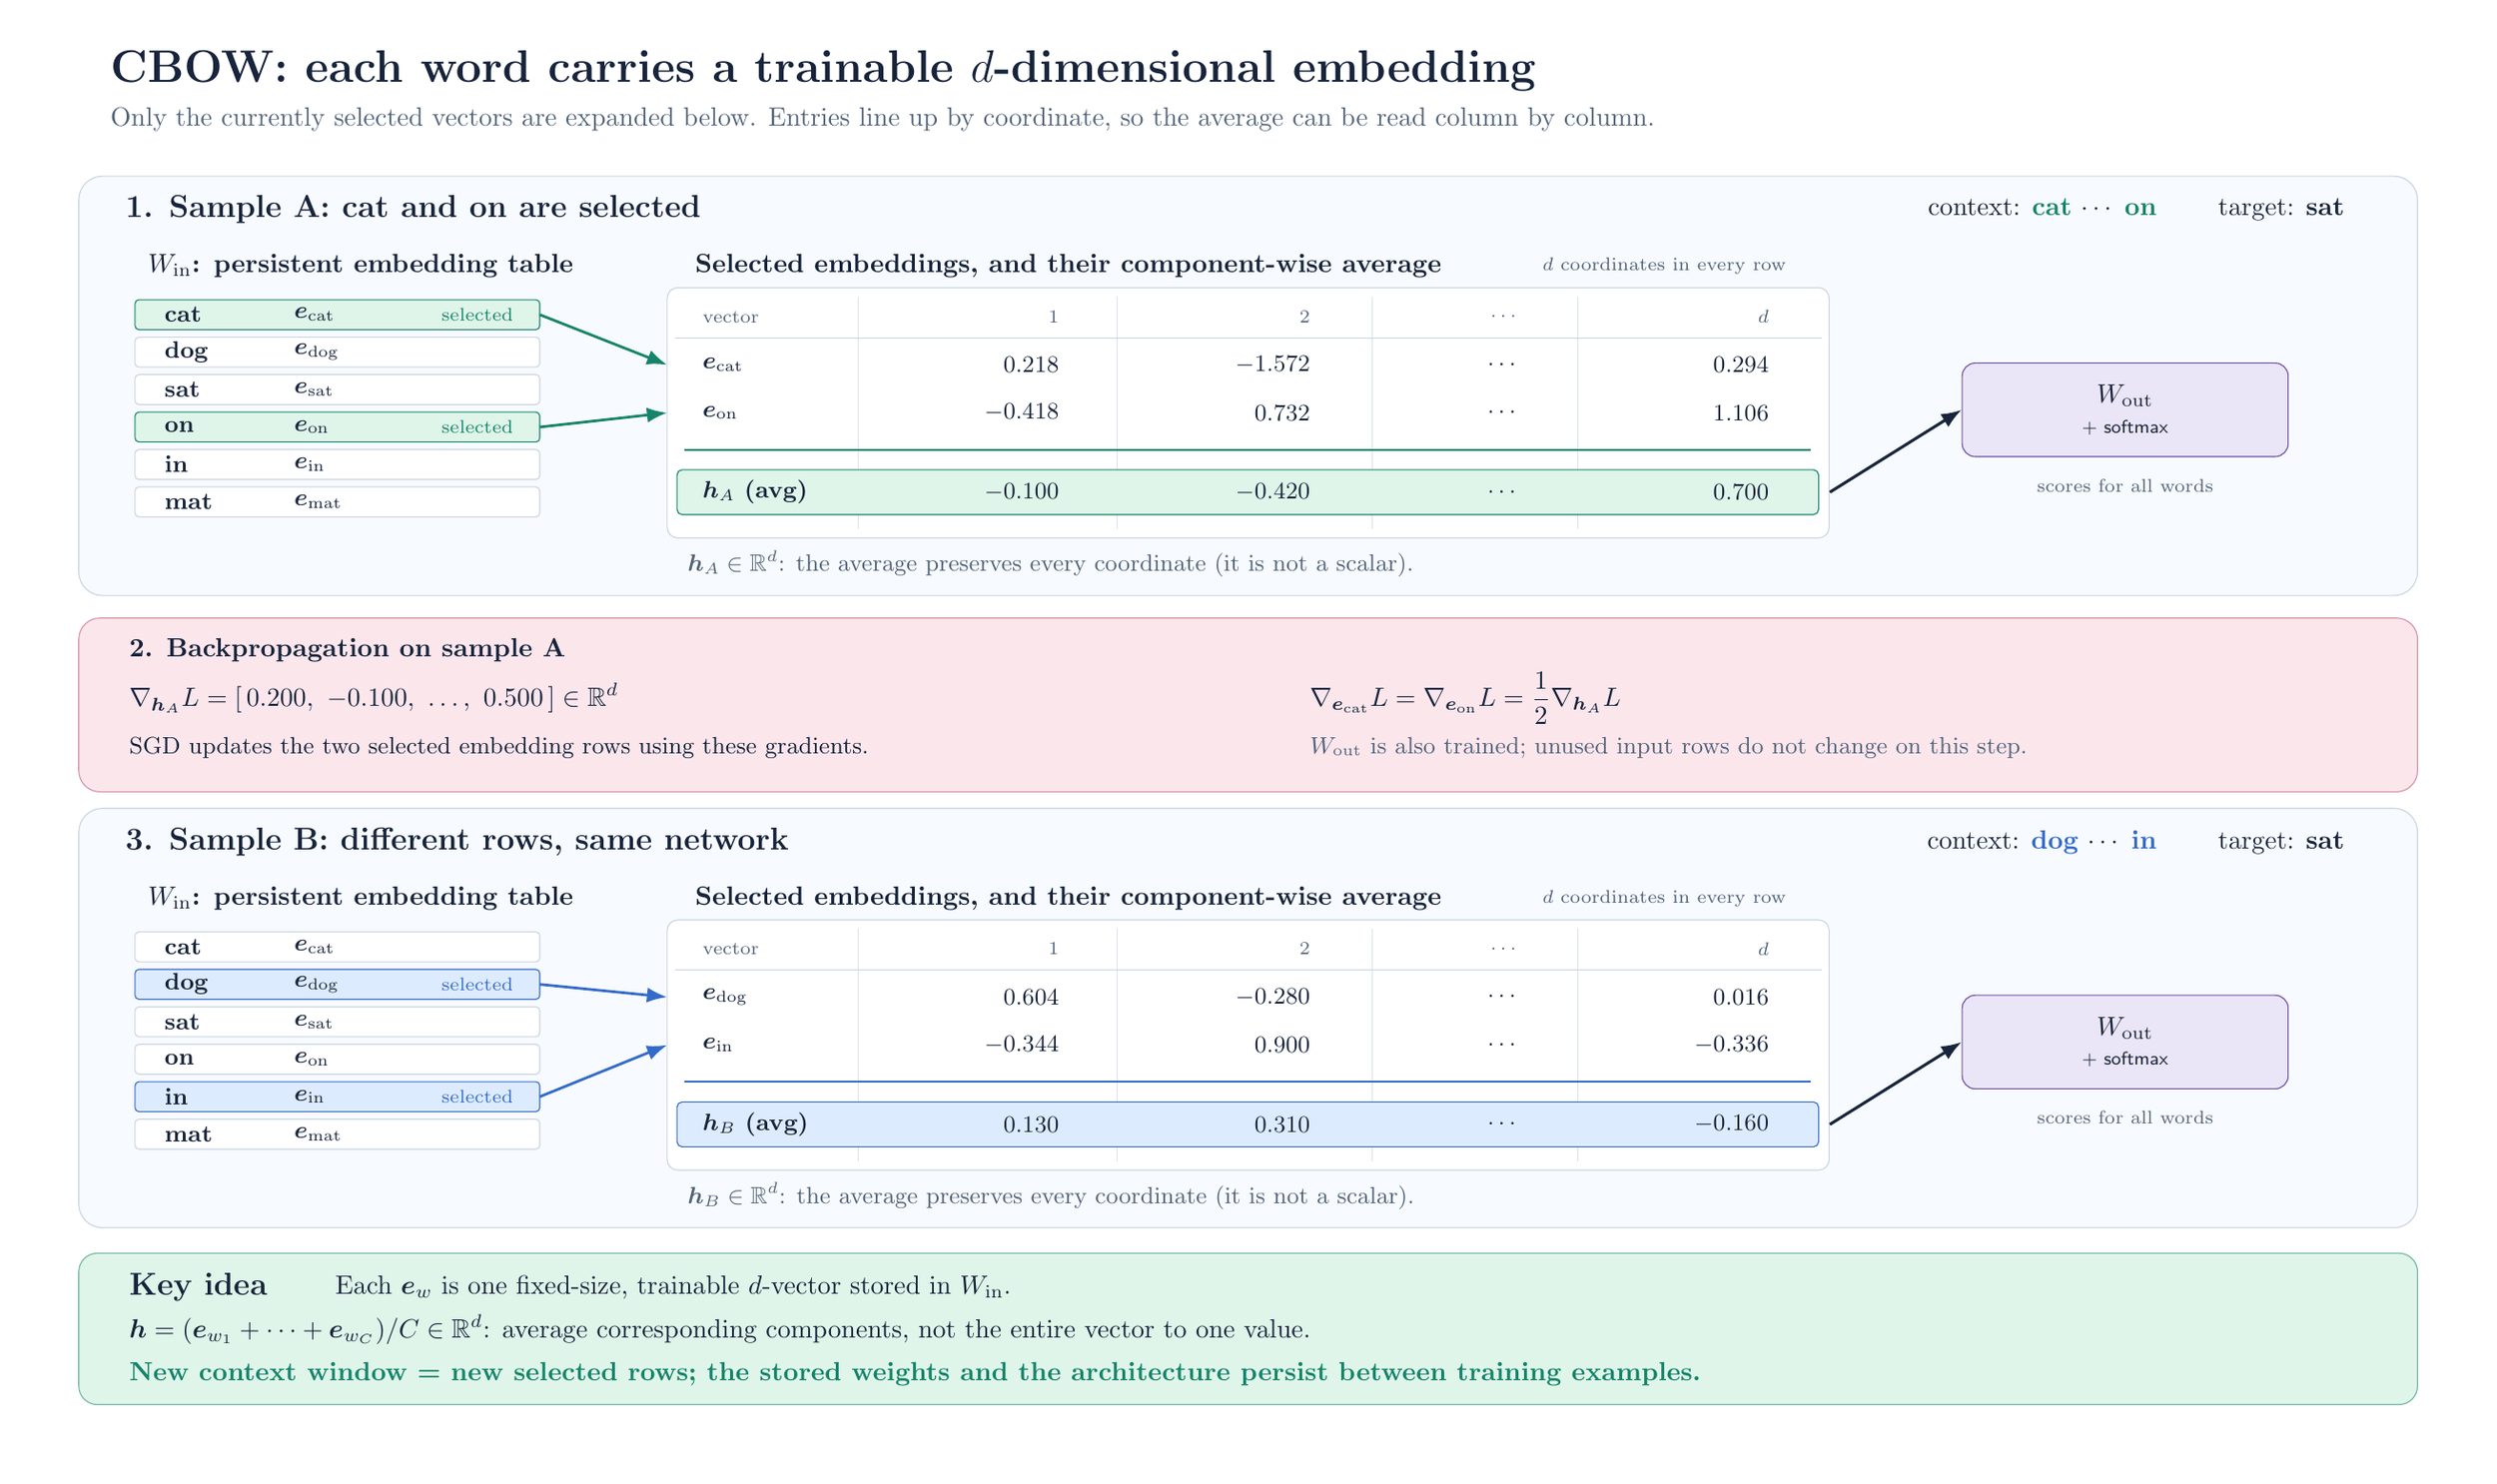
\begin{tikzpicture}[x=1cm,y=1cm,font=\sffamily,text=ink]
\fill[white] (0,0) rectangle (32.6,19.1);
\node[anchor=west,font=\bfseries\LARGE] at (1.0,18.50)
  {CBOW: each word carries a trainable $d$-dimensional embedding};
\node[anchor=west,font=\normalsize,text=muted] at (1.0,17.86)
  {Only the currently selected vectors are expanded below. Entries line up by coordinate, so the average can be read column by column.};
\filldraw[draw=line,fill=panelbg,rounded corners=9pt] (0.70,11.50) rectangle (31.90,17.10);
\node[anchor=west,font=\bfseries\large] at (1.20,16.65) {1. Sample A: cat and on are selected};
\node[anchor=east,font=\normalsize] at (31.05,16.65) {context: \textcolor{teal}{\textbf{cat}} $\cdots$ \textcolor{teal}{\textbf{on}} \qquad target: \textbf{sat}};
\node[anchor=west,font=\bfseries\normalsize] at (1.50,15.90) {$W_{\rm in}$: persistent embedding table};
\node[anchor=west,font=\bfseries\normalsize] at (8.80,15.90) {Selected embeddings, and their component-wise average};
\node[anchor=east,font=\scriptsize,text=muted] at (23.60,15.90) {$d$ coordinates in every row};
\filldraw[fill=selectA,draw=teal,rounded corners=1.5pt] (1.45,15.05) rectangle (6.85,15.45);
\node[anchor=west,font=\small\bfseries] at (1.72,15.25) {cat};
\node[anchor=west,font=\small] at (3.45,15.25) {$\boldsymbol e_{\rm cat}$};
\node[anchor=east,font=\scriptsize,text=teal] at (6.62,15.25) {selected};
\filldraw[fill=white,draw=line,rounded corners=1.5pt] (1.45,14.55) rectangle (6.85,14.95);
\node[anchor=west,font=\small\bfseries] at (1.72,14.75) {dog};
\node[anchor=west,font=\small] at (3.45,14.75) {$\boldsymbol e_{\rm dog}$};
\filldraw[fill=white,draw=line,rounded corners=1.5pt] (1.45,14.05) rectangle (6.85,14.45);
\node[anchor=west,font=\small\bfseries] at (1.72,14.25) {sat};
\node[anchor=west,font=\small] at (3.45,14.25) {$\boldsymbol e_{\rm sat}$};
\filldraw[fill=selectA,draw=teal,rounded corners=1.5pt] (1.45,13.55) rectangle (6.85,13.95);
\node[anchor=west,font=\small\bfseries] at (1.72,13.75) {on};
\node[anchor=west,font=\small] at (3.45,13.75) {$\boldsymbol e_{\rm on}$};
\node[anchor=east,font=\scriptsize,text=teal] at (6.62,13.75) {selected};
\filldraw[fill=white,draw=line,rounded corners=1.5pt] (1.45,13.05) rectangle (6.85,13.45);
\node[anchor=west,font=\small\bfseries] at (1.72,13.25) {in};
\node[anchor=west,font=\small] at (3.45,13.25) {$\boldsymbol e_{\rm in}$};
\filldraw[fill=white,draw=line,rounded corners=1.5pt] (1.45,12.55) rectangle (6.85,12.95);
\node[anchor=west,font=\small\bfseries] at (1.72,12.75) {mat};
\node[anchor=west,font=\small] at (3.45,12.75) {$\boldsymbol e_{\rm mat}$};
\filldraw[draw=line,fill=white,rounded corners=4pt] (8.55,12.27) rectangle (24.05,15.61);
\draw[draw=line!70,line width=.3pt] (11.10,12.39) -- (11.10,15.49);
\draw[draw=line!70,line width=.3pt] (14.55,12.39) -- (14.55,15.49);
\draw[draw=line!70,line width=.3pt] (17.96,12.39) -- (17.96,15.49);
\draw[draw=line!70,line width=.3pt] (20.70,12.39) -- (20.70,15.49);
\node[anchor=west,font=\scriptsize,text=muted] at (8.90,15.22) {vector};
\node[anchor=east,font=\scriptsize,text=muted] at (13.90,15.22) {$1$};
\node[anchor=east,font=\scriptsize,text=muted] at (17.25,15.22) {$2$};
\node[anchor=east,font=\scriptsize,text=muted] at (20.05,15.22) {$\cdots$};
\node[anchor=east,font=\scriptsize,text=muted] at (23.37,15.22) {$d$};
\draw[draw=line,line width=.5pt] (8.65,14.94) -- (23.95,14.94);
\node[anchor=west,font=\small\bfseries] at (8.90,14.58) {$\boldsymbol e_{\rm cat}$};
\node[anchor=east,font=\small] at (13.90,14.58) {$0.218$};
\node[anchor=east,font=\small] at (17.25,14.58) {$-1.572$};
\node[anchor=east,font=\small] at (20.05,14.58) {$\cdots$};
\node[anchor=east,font=\small] at (23.37,14.58) {$0.294$};
\node[anchor=west,font=\small\bfseries] at (8.90,13.94) {$\boldsymbol e_{\rm on}$};
\node[anchor=east,font=\small] at (13.90,13.94) {$-0.418$};
\node[anchor=east,font=\small] at (17.25,13.94) {$0.732$};
\node[anchor=east,font=\small] at (20.05,13.94) {$\cdots$};
\node[anchor=east,font=\small] at (23.37,13.94) {$1.106$};
\filldraw[draw=teal,fill=selectA,rounded corners=2pt] (8.68,12.58) rectangle (23.91,13.18);
\node[anchor=west,font=\small\bfseries] at (8.90,12.88) {$\boldsymbol h_{A}$ (avg)};
\node[anchor=east,font=\small] at (13.90,12.88) {$-0.100$};
\node[anchor=east,font=\small] at (17.25,12.88) {$-0.420$};
\node[anchor=east,font=\small] at (20.05,12.88) {$\cdots$};
\node[anchor=east,font=\small] at (23.37,12.88) {$0.700$};
\draw[draw=teal,line width=.7pt] (8.78,13.45) -- (23.8,13.45);

\draw[->,draw=teal,line width=1.0pt] (6.85,15.25) -- (8.55,14.58);
\draw[->,draw=teal,line width=1.0pt] (6.85,13.75) -- (8.55,13.94);
\node[classifier,minimum height=1.25cm,minimum width=4.35cm] (outA) at (28.00,13.98) {$W_{\rm out}$\\[-.2mm]\scriptsize + softmax};
\draw[flow] (24.06,12.88) -- (outA.west);
\node[anchor=north,font=\scriptsize,text=muted] at (28.0,13.18) {scores for all words};
\node[anchor=west,font=\small,text=muted] at (8.70,11.92) {$\boldsymbol h_{A}\in\mathbb R^d$: the average preserves every coordinate (it is not a scalar).};

% Mid-page gradient strip
\filldraw[draw=pink!55,fill=palepink,rounded corners=8pt] (0.70,8.88) rectangle (31.90,11.20);
\node[anchor=west,font=\bfseries\normalsize] at (1.25,10.77)
  {2. Backpropagation on sample A};
\node[anchor=west,font=\normalsize] at (1.25,10.13)
  {$\displaystyle \nabla_{\boldsymbol h_A}L=[\,0.200,\ -0.100,\ \ldots,\ 0.500\,]\in\mathbb R^d$};
\node[anchor=west,font=\normalsize] at (17.00,10.13)
  {$\displaystyle \nabla_{\boldsymbol e_{\rm cat}}L=\nabla_{\boldsymbol e_{\rm on}}L=\frac12\nabla_{\boldsymbol h_A}L$};
\node[anchor=west,font=\small] at (1.25,9.47)
  {SGD updates the two selected embedding rows using these gradients.};
\node[anchor=west,font=\small,text=muted] at (17.00,9.47)
  {$W_{\rm out}$ is also trained; unused input rows do not change on this step.};
\filldraw[draw=line,fill=panelbg,rounded corners=9pt] (0.70,3.06) rectangle (31.90,8.66);
\node[anchor=west,font=\bfseries\large] at (1.20,8.21) {3. Sample B: different rows, same network};
\node[anchor=east,font=\normalsize] at (31.05,8.21) {context: \textcolor{blue}{\textbf{dog}} $\cdots$ \textcolor{blue}{\textbf{in}} \qquad target: \textbf{sat}};
\node[anchor=west,font=\bfseries\normalsize] at (1.50,7.46) {$W_{\rm in}$: persistent embedding table};
\node[anchor=west,font=\bfseries\normalsize] at (8.80,7.46) {Selected embeddings, and their component-wise average};
\node[anchor=east,font=\scriptsize,text=muted] at (23.60,7.46) {$d$ coordinates in every row};
\filldraw[fill=white,draw=line,rounded corners=1.5pt] (1.45,6.61) rectangle (6.85,7.01);
\node[anchor=west,font=\small\bfseries] at (1.72,6.81) {cat};
\node[anchor=west,font=\small] at (3.45,6.81) {$\boldsymbol e_{\rm cat}$};
\filldraw[fill=selectB,draw=blue,rounded corners=1.5pt] (1.45,6.11) rectangle (6.85,6.51);
\node[anchor=west,font=\small\bfseries] at (1.72,6.31) {dog};
\node[anchor=west,font=\small] at (3.45,6.31) {$\boldsymbol e_{\rm dog}$};
\node[anchor=east,font=\scriptsize,text=blue] at (6.62,6.31) {selected};
\filldraw[fill=white,draw=line,rounded corners=1.5pt] (1.45,5.61) rectangle (6.85,6.01);
\node[anchor=west,font=\small\bfseries] at (1.72,5.81) {sat};
\node[anchor=west,font=\small] at (3.45,5.81) {$\boldsymbol e_{\rm sat}$};
\filldraw[fill=white,draw=line,rounded corners=1.5pt] (1.45,5.11) rectangle (6.85,5.51);
\node[anchor=west,font=\small\bfseries] at (1.72,5.31) {on};
\node[anchor=west,font=\small] at (3.45,5.31) {$\boldsymbol e_{\rm on}$};
\filldraw[fill=selectB,draw=blue,rounded corners=1.5pt] (1.45,4.61) rectangle (6.85,5.01);
\node[anchor=west,font=\small\bfseries] at (1.72,4.81) {in};
\node[anchor=west,font=\small] at (3.45,4.81) {$\boldsymbol e_{\rm in}$};
\node[anchor=east,font=\scriptsize,text=blue] at (6.62,4.81) {selected};
\filldraw[fill=white,draw=line,rounded corners=1.5pt] (1.45,4.11) rectangle (6.85,4.51);
\node[anchor=west,font=\small\bfseries] at (1.72,4.31) {mat};
\node[anchor=west,font=\small] at (3.45,4.31) {$\boldsymbol e_{\rm mat}$};
\filldraw[draw=line,fill=white,rounded corners=4pt] (8.55,3.83) rectangle (24.05,7.17);
\draw[draw=line!70,line width=.3pt] (11.10,3.95) -- (11.10,7.05);
\draw[draw=line!70,line width=.3pt] (14.55,3.95) -- (14.55,7.05);
\draw[draw=line!70,line width=.3pt] (17.96,3.95) -- (17.96,7.05);
\draw[draw=line!70,line width=.3pt] (20.70,3.95) -- (20.70,7.05);
\node[anchor=west,font=\scriptsize,text=muted] at (8.90,6.78) {vector};
\node[anchor=east,font=\scriptsize,text=muted] at (13.90,6.78) {$1$};
\node[anchor=east,font=\scriptsize,text=muted] at (17.25,6.78) {$2$};
\node[anchor=east,font=\scriptsize,text=muted] at (20.05,6.78) {$\cdots$};
\node[anchor=east,font=\scriptsize,text=muted] at (23.37,6.78) {$d$};
\draw[draw=line,line width=.5pt] (8.65,6.50) -- (23.95,6.50);
\node[anchor=west,font=\small\bfseries] at (8.90,6.14) {$\boldsymbol e_{\rm dog}$};
\node[anchor=east,font=\small] at (13.90,6.14) {$0.604$};
\node[anchor=east,font=\small] at (17.25,6.14) {$-0.280$};
\node[anchor=east,font=\small] at (20.05,6.14) {$\cdots$};
\node[anchor=east,font=\small] at (23.37,6.14) {$0.016$};
\node[anchor=west,font=\small\bfseries] at (8.90,5.50) {$\boldsymbol e_{\rm in}$};
\node[anchor=east,font=\small] at (13.90,5.50) {$-0.344$};
\node[anchor=east,font=\small] at (17.25,5.50) {$0.900$};
\node[anchor=east,font=\small] at (20.05,5.50) {$\cdots$};
\node[anchor=east,font=\small] at (23.37,5.50) {$-0.336$};
\filldraw[draw=blue,fill=selectB,rounded corners=2pt] (8.68,4.14) rectangle (23.91,4.74);
\node[anchor=west,font=\small\bfseries] at (8.90,4.44) {$\boldsymbol h_{B}$ (avg)};
\node[anchor=east,font=\small] at (13.90,4.44) {$0.130$};
\node[anchor=east,font=\small] at (17.25,4.44) {$0.310$};
\node[anchor=east,font=\small] at (20.05,4.44) {$\cdots$};
\node[anchor=east,font=\small] at (23.37,4.44) {$-0.160$};
\draw[draw=blue,line width=.7pt] (8.78,5.01) -- (23.8,5.01);

\draw[->,draw=blue,line width=1.0pt] (6.85,6.31) -- (8.55,6.14);
\draw[->,draw=blue,line width=1.0pt] (6.85,4.81) -- (8.55,5.50);
\node[classifier,minimum height=1.25cm,minimum width=4.35cm] (outB) at (28.00,5.54) {$W_{\rm out}$\\[-.2mm]\scriptsize + softmax};
\draw[flow] (24.06,4.44) -- (outB.west);
\node[anchor=north,font=\scriptsize,text=muted] at (28.0,4.74) {scores for all words};
\node[anchor=west,font=\small,text=muted] at (8.70,3.48) {$\boldsymbol h_{B}\in\mathbb R^d$: the average preserves every coordinate (it is not a scalar).};

% Compact takeaway with sufficient whitespace
\filldraw[draw=teal!60,fill=selectA,rounded corners=7pt] (0.7,0.70) rectangle (31.9,2.72);
\node[anchor=west,font=\bfseries\large] at (1.25,2.26) {Key idea};
\node[anchor=west,font=\normalsize] at (4.0,2.26)
  {Each $\boldsymbol e_w$ is one fixed-size, trainable $d$-vector stored in $W_{\rm in}$.};
\node[anchor=west,font=\normalsize] at (1.25,1.70)
  {$\boldsymbol h=(\boldsymbol e_{w_1}+\cdots+\boldsymbol e_{w_C})/C\in\mathbb R^d$: average corresponding components, not the entire vector to one value.};
\node[anchor=west,font=\bfseries\normalsize,text=teal] at (1.25,1.10)
  {New context window = new selected rows; the stored weights and the architecture persist between training examples.};
\end{tikzpicture}

% === Page 3: high-level explanation with a separated training flow. ===
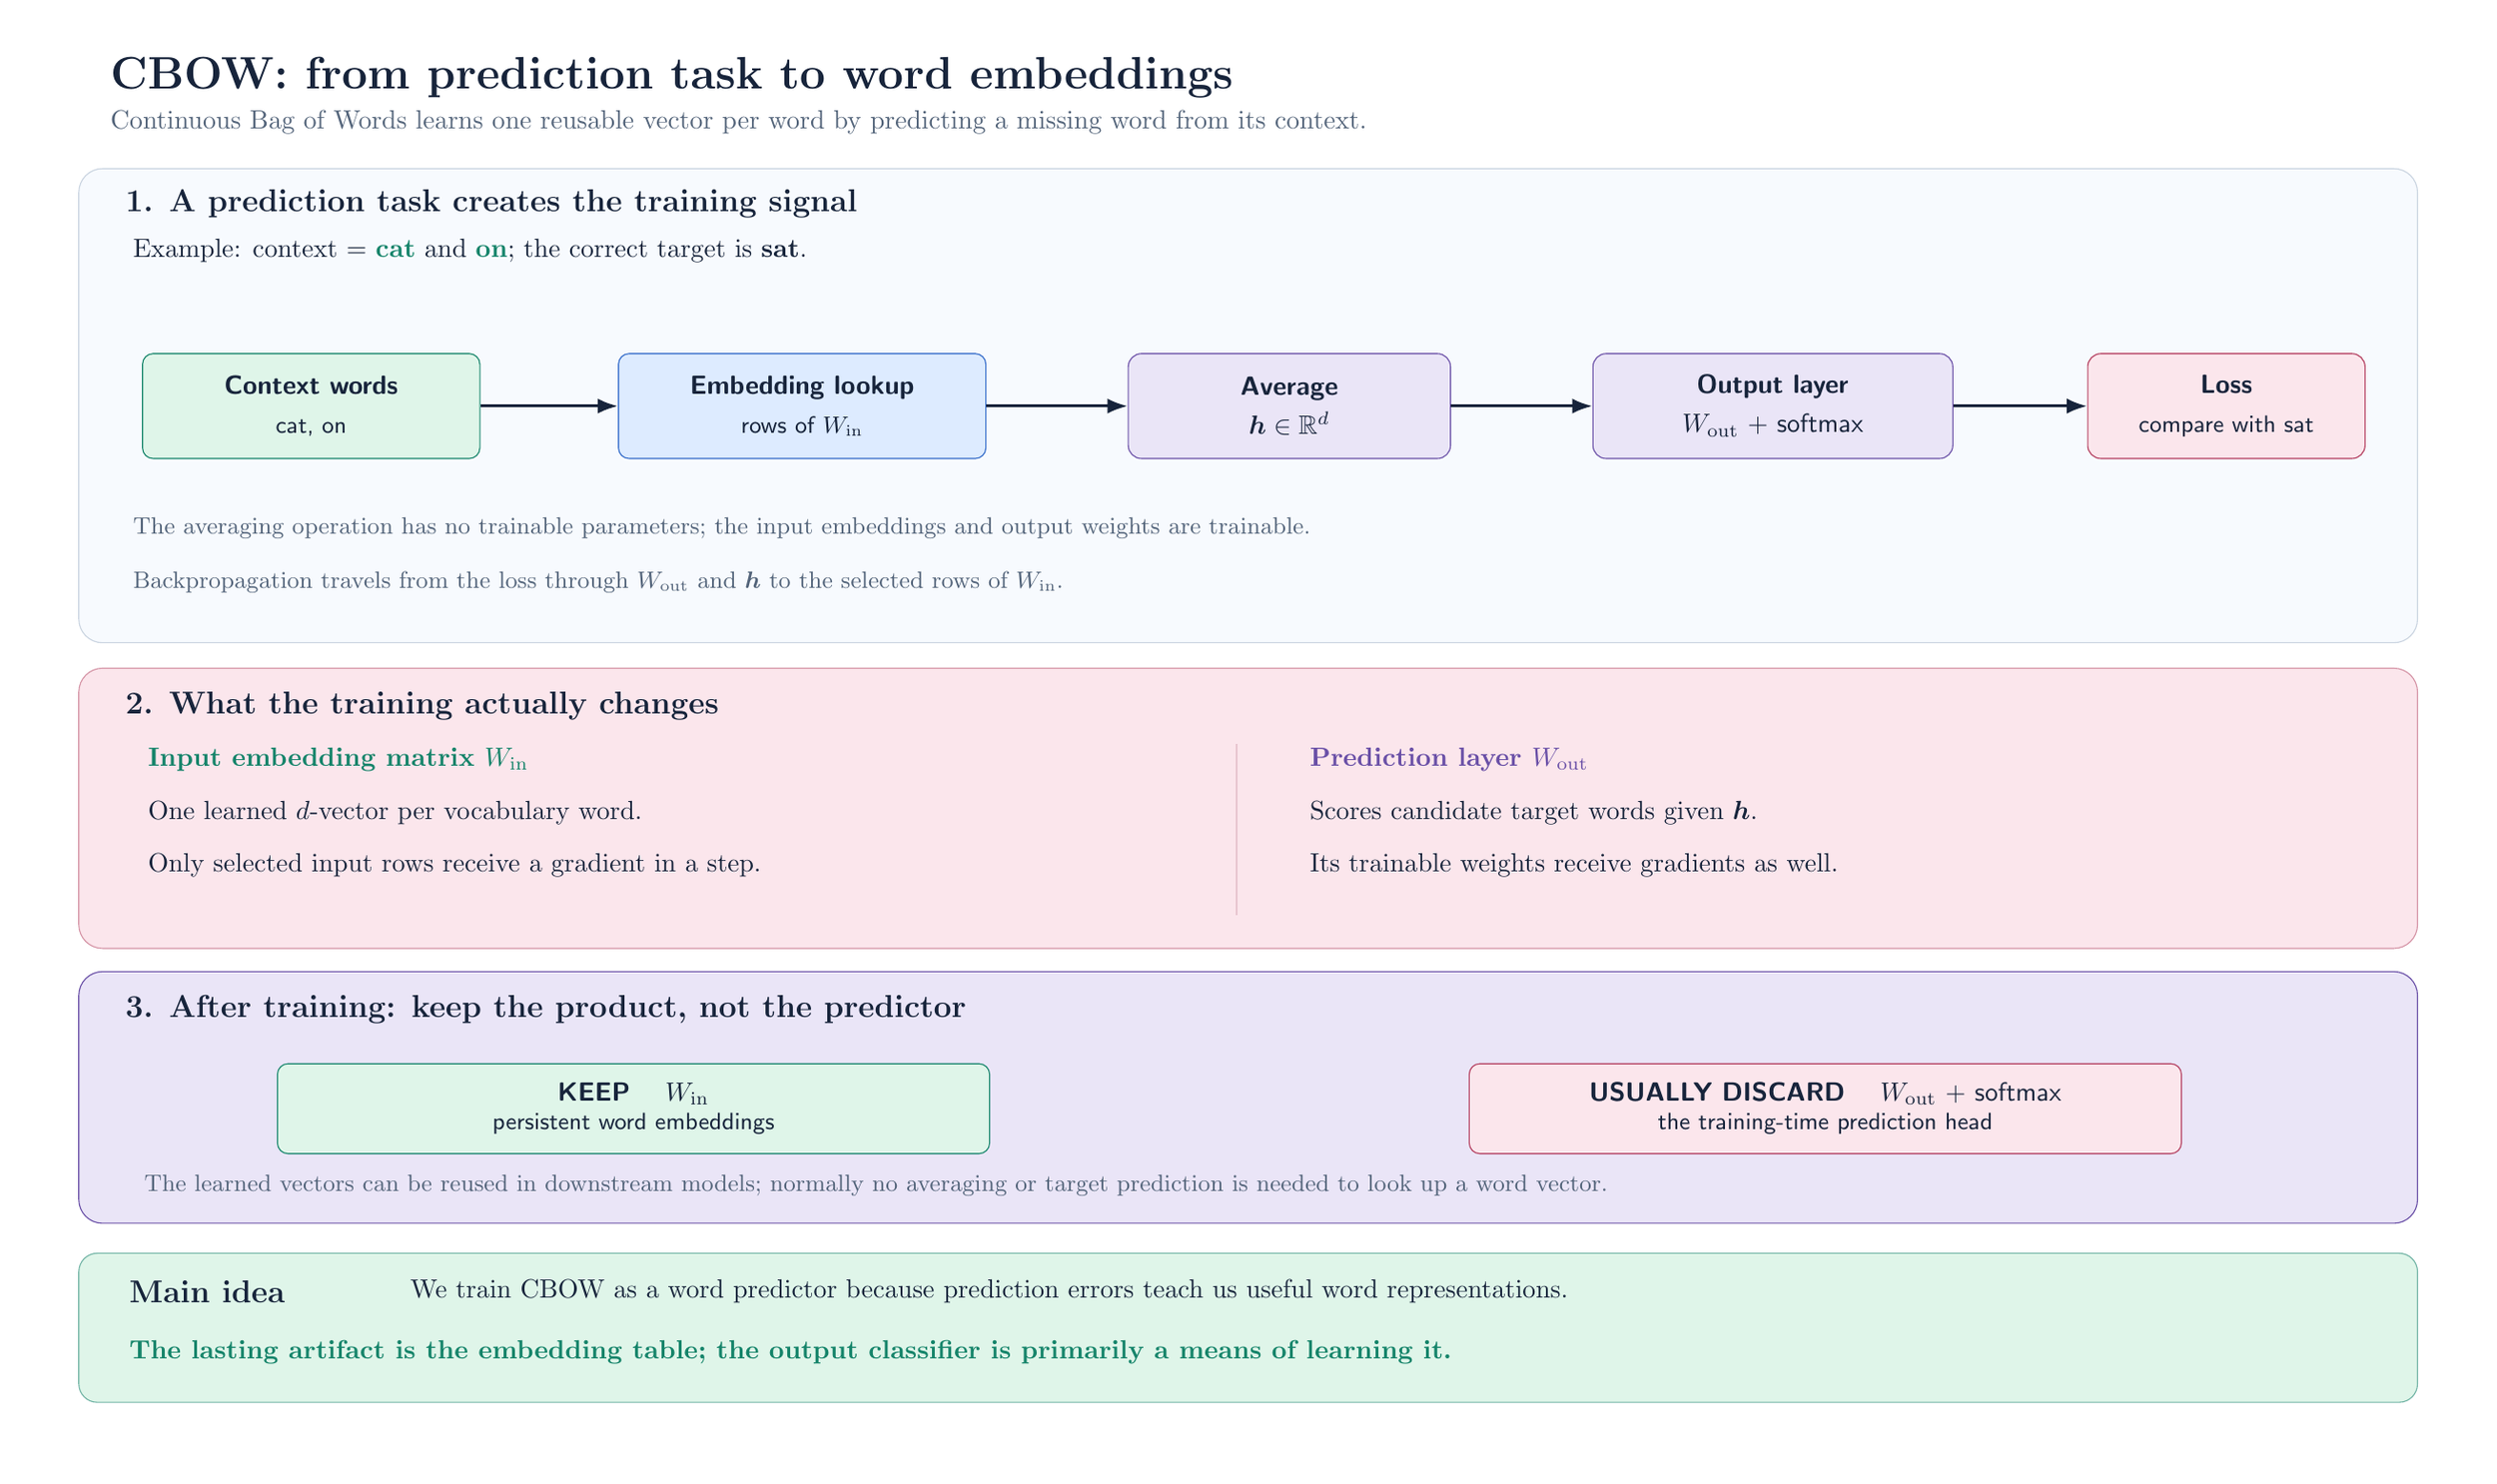
\begin{tikzpicture}[x=1cm,y=1cm,font=\sffamily,text=ink]
\fill[white] (0,0) rectangle (32.6,19.1);
\node[anchor=west,font=\bfseries\LARGE] at (1.0,18.42) {CBOW: from prediction task to word embeddings};
\node[anchor=west,font=\normalsize,text=muted] at (1.0,17.82)
  {Continuous Bag of Words learns one reusable vector per word by predicting a missing word from its context.};

% 1 - carefully separated pipeline
\filldraw[draw=line,fill=panelbg,rounded corners=9pt] (0.7,10.87) rectangle (31.9,17.20);
\node[anchor=west,font=\bfseries\large] at (1.20,16.73) {1. A prediction task creates the training signal};
\node[anchor=west,font=\normalsize] at (1.30,16.10)
  {Example: context = \textcolor{teal}{\textbf{cat}} and \textcolor{teal}{\textbf{on}}; the correct target is \textbf{sat}.};

\node[box,draw=teal,fill=selectA,minimum width=4.5cm,minimum height=1.40cm] (p3ctx) at (3.80,14.03)
  {\textbf{Context words}\\[1mm]\small cat, on};
\node[box,draw=blue,fill=selectB,minimum width=4.90cm,minimum height=1.40cm] (p3emb) at (10.35,14.03)
  {\textbf{Embedding lookup}\\[1mm]\small rows of $W_{\rm in}$};
\node[avg,minimum width=4.30cm,minimum height=1.40cm] (p3mean) at (16.85,14.03)
  {\textbf{Average}\\[1mm]$\boldsymbol h\in\mathbb R^d$};
\node[classifier,minimum width=4.80cm,minimum height=1.40cm] (p3head) at (23.30,14.03)
  {\textbf{Output layer}\\[1mm]$W_{\rm out}$ + softmax};
\node[target,minimum width=3.7cm,minimum height=1.40cm] (p3target) at (29.35,14.03)
  {\textbf{Loss}\\[1mm]\small compare with sat};
\draw[flow] (p3ctx.east) -- (p3emb.west);
\draw[flow] (p3emb.east) -- (p3mean.west);
\draw[flow] (p3mean.east) -- (p3head.west);
\draw[flow] (p3head.east) -- (p3target.west);
\node[anchor=west,font=\small,text=muted] at (1.30,12.40)
  {The averaging operation has no trainable parameters; the input embeddings and output weights are trainable.};
\node[anchor=west,font=\small,text=muted] at (1.30,11.67)
  {Backpropagation travels from the loss through $W_{\rm out}$ and $\boldsymbol h$ to the selected rows of $W_{\rm in}$.};

% 2 - two columns of statements
\filldraw[draw=pink!55,fill=palepink,rounded corners=9pt] (0.7,6.79) rectangle (31.9,10.53);
\node[anchor=west,font=\bfseries\large] at (1.20,10.03) {2. What the training actually changes};
\draw[draw=pink!30,line width=0.7pt] (16.15,7.23) -- (16.15,9.52);
\node[anchor=west,font=\bfseries\normalsize,text=teal] at (1.50,9.31) {Input embedding matrix $W_{\rm in}$};
\node[anchor=west,font=\normalsize] at (1.50,8.60) {One learned $d$-vector per vocabulary word.};
\node[anchor=west,font=\normalsize] at (1.50,7.90) {Only selected input rows receive a gradient in a step.};
\node[anchor=west,font=\bfseries\normalsize,text=violet] at (17.0,9.31) {Prediction layer $W_{\rm out}$};
\node[anchor=west,font=\normalsize] at (17.0,8.60) {Scores candidate target words given $\boldsymbol h$.};
\node[anchor=west,font=\normalsize] at (17.0,7.90) {Its trainable weights receive gradients as well.};

% 3 - use-stage result without overlap
\filldraw[draw=violet,fill=paleviolet,rounded corners=9pt] (0.7,3.12) rectangle (31.9,6.48);
\node[anchor=west,font=\bfseries\large] at (1.20,5.98) {3. After training: keep the product, not the predictor};
\node[box,draw=teal,fill=selectA,minimum width=9.5cm,minimum height=1.20cm] (p3keep)
  at (8.1,4.65) {\textbf{KEEP} $\quad W_{\rm in}$\\[-0.4mm]\small persistent word embeddings};
\node[box,draw=pink,fill=palepink,minimum width=9.5cm,minimum height=1.20cm] (p3discard)
  at (24.0,4.65) {\textbf{USUALLY DISCARD} $\quad W_{\rm out}$ + softmax\\[-0.4mm]\small the training-time prediction head};
\node[anchor=west,font=\small,text=muted] at (1.45,3.63)
  {The learned vectors can be reused in downstream models; normally no averaging or target prediction is needed to look up a word vector.};

% Summary
\filldraw[draw=teal!60,fill=selectA,rounded corners=7pt] (0.7,0.73) rectangle (31.9,2.72);
\node[anchor=west,font=\bfseries\large] at (1.25,2.21) {Main idea};
\node[anchor=west,font=\normalsize] at (5.0,2.21)
  {We train CBOW as a word predictor because prediction errors teach us useful word representations.};
\node[anchor=west,font=\bfseries\normalsize,text=teal] at (1.25,1.40)
  {The lasting artifact is the embedding table; the output classifier is primarily a means of learning it.};
\end{tikzpicture}



% ============ PAGE 4: MATRIX FORMULATION, C = 7 ============
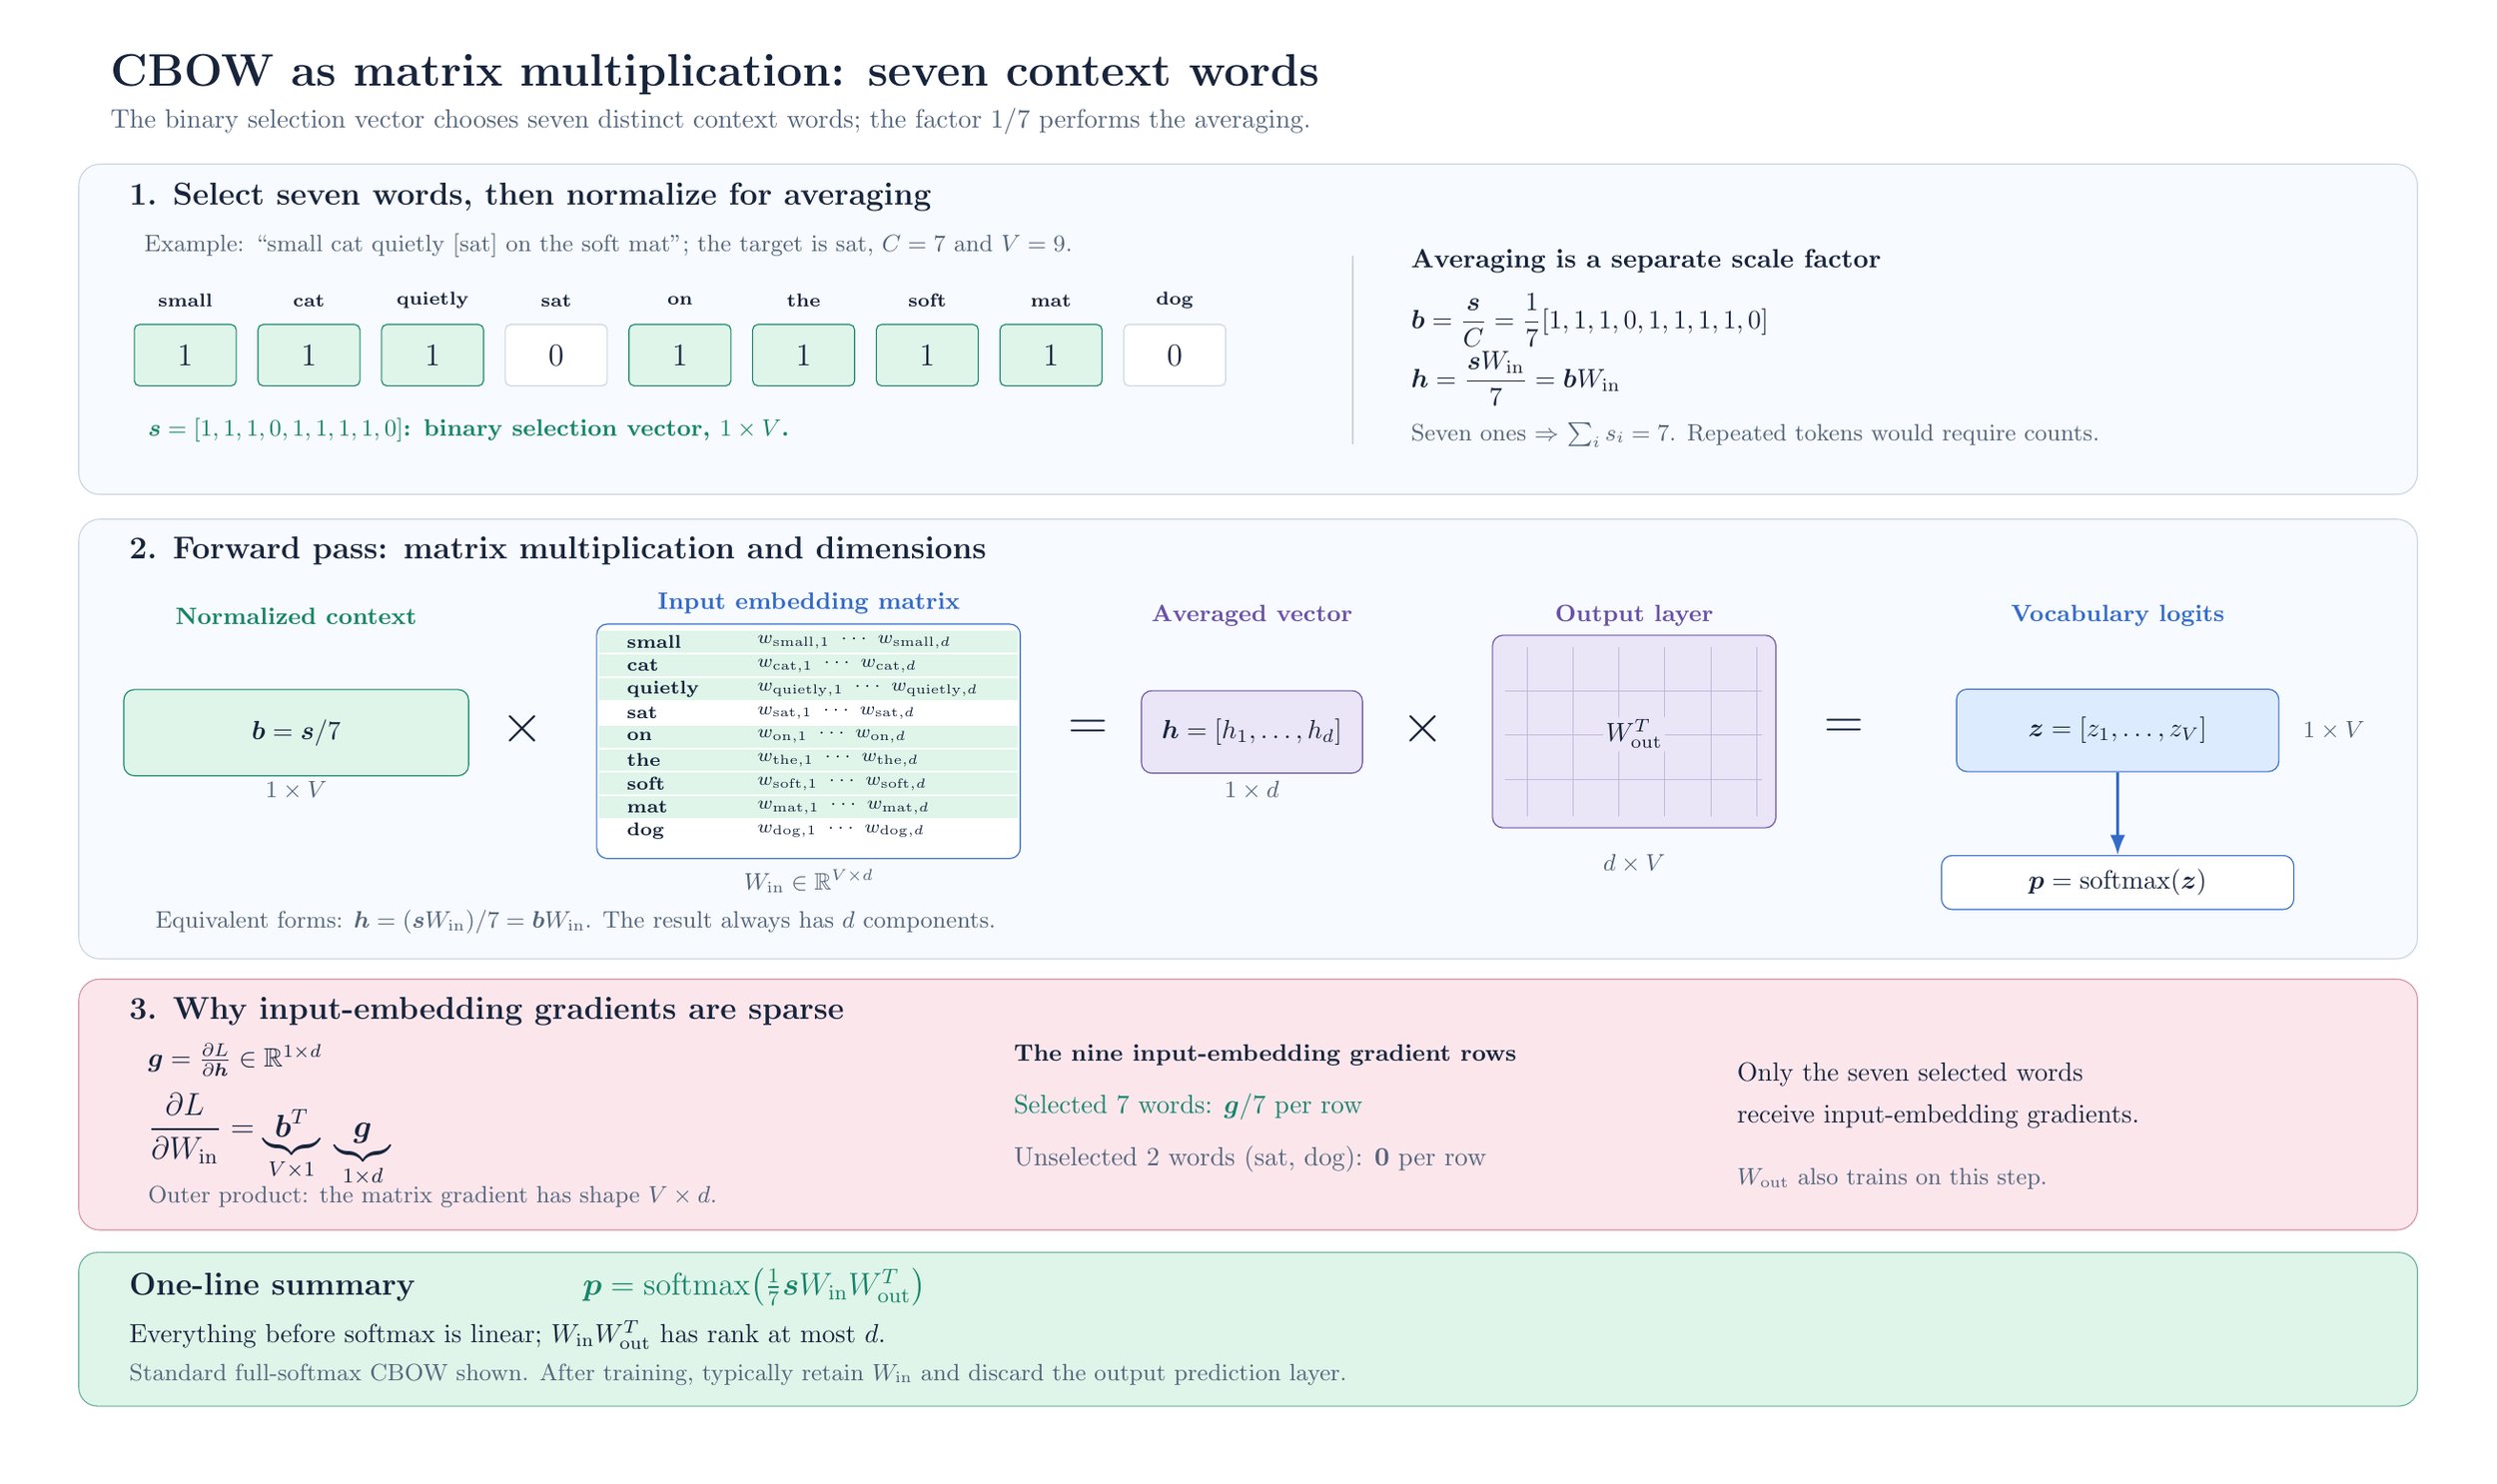
\begin{tikzpicture}[x=1cm,y=1cm,font=\sffamily,text=ink]
\fill[white] (0,0) rectangle (32.6,19.1);
\node[anchor=west,font=\bfseries\LARGE] at (1.0,18.45)
  {CBOW as matrix multiplication: seven context words};
\node[anchor=west,font=\normalsize,text=muted] at (1.0,17.83)
  {The binary selection vector chooses seven distinct context words; the factor $1/7$ performs the averaging.};

% SECTION 1: BINARY SELECTION, C=7
\filldraw[draw=line,fill=panelbg,rounded corners=8pt] (0.7,12.85) rectangle (31.9,17.26);
\node[anchor=west,font=\bfseries\large] at (1.25,16.82) {1. Select seven words, then normalize for averaging};
\node[anchor=west,font=\small,text=muted] at (1.45,16.17)
  {Example: ``small cat quietly [sat] on the soft mat''; the target is sat, $C=7$ and $V=9$.};

% Selection vector (one column per word, exactly seven ones)
\foreach \w/\idx/\flag in {small/0/1,cat/1/1,quietly/2/1,sat/3/0,on/4/1,the/5/1,soft/6/1,mat/7/1,dog/8/0}{
  \pgfmathsetmacro{\xx}{2.12+1.65*\idx}
  \node[font=\scriptsize\bfseries] at (\xx,15.44) {\w};
  \ifnum\flag=1
    \filldraw[draw=teal,fill=selectA,rounded corners=2pt] (\xx-0.68,14.30) rectangle (\xx+0.68,15.12);
  \else
    \filldraw[draw=line,fill=white,rounded corners=2pt] (\xx-0.68,14.30) rectangle (\xx+0.68,15.12);
  \fi
  \node[font=\large] at (\xx,14.71) {$\flag$};
}
\node[anchor=west,font=\small\bfseries,text=teal] at (1.50,13.71)
  {$\boldsymbol s=[1,1,1,0,1,1,1,1,0]$: binary selection vector, $1\times V$.};
\draw[draw=line,line width=.7pt] (17.70,13.52)--(17.70,16.04);
\node[anchor=west,font=\bfseries\normalsize] at (18.35,15.96) {Averaging is a separate scale factor};
\node[anchor=west,font=\normalsize] at (18.35,15.18)
  {$\displaystyle \boldsymbol b=\frac{\boldsymbol s}{C}=\frac17[1,1,1,0,1,1,1,1,0]$};
\node[anchor=west,font=\normalsize] at (18.35,14.40)
  {$\displaystyle \boldsymbol h=\frac{\boldsymbol sW_{\rm in}}7=\boldsymbol bW_{\rm in}$};
\node[anchor=west,font=\small,text=muted] at (18.35,13.64)
  {Seven ones $\Rightarrow$ $\sum_i s_i=7$. Repeated tokens would require counts.};

% SECTION 2: MAIN MATRIX PIPELINE
\filldraw[draw=line,fill=panelbg,rounded corners=8pt] (0.7,6.65) rectangle (31.9,12.52);
\node[anchor=west,font=\bfseries\large] at (1.25,12.09) {2. Forward pass: matrix multiplication and dimensions};
\node[font=\bfseries\small,text=teal] at (3.60,11.23) {Normalized context};
\node[box,draw=teal,fill=selectA,minimum width=4.6cm,minimum height=1.15cm] at (3.60,9.67)
  {$\boldsymbol b=\boldsymbol s/7$};
\node[font=\small,text=muted] at (3.60,8.90) {$1\times V$};
\node[font=\huge] at (6.62,9.72) {$\times$};
\node[font=\bfseries\small,text=blue] at (10.44,11.39) {Input embedding matrix};
\filldraw[draw=blue,fill=white,rounded corners=4pt] (7.61,7.99) rectangle (13.26,11.12);
\foreach \w/\idx/\flag in {small/0/1,cat/1/1,quietly/2/1,sat/3/0,on/4/1,the/5/1,soft/6/1,mat/7/1,dog/8/0}{
  \pgfmathsetmacro{\yy}{10.88-0.315*\idx}
  \ifnum\flag=1
    \fill[selectA] (7.64,\yy-0.145) rectangle (13.22,\yy+0.145);
  \fi
  \node[anchor=west,font=\scriptsize\bfseries] at (7.89,\yy) {\w};
  \node[anchor=west,font=\scriptsize] at (9.63,\yy) {$w_{\mathrm{\w},1}\ \cdots\ w_{\mathrm{\w},d}$};
}
\node[font=\small,text=muted] at (10.44,7.69) {$W_{\rm in}\in\mathbb R^{V\times d}$};
\node[font=\huge] at (14.17,9.71) {$=$};
\node[font=\bfseries\small,text=violet] at (16.35,11.23) {Averaged vector};
\node[box,draw=violet,fill=paleviolet,minimum width=2.95cm,minimum height=1.1cm] at (16.35,9.68)
  {$\boldsymbol h=[h_1,\ldots,h_d]$};
\node[font=\small,text=muted] at (16.35,8.90) {$1\times d$};
\node[font=\huge] at (18.63,9.72) {$\times$};
\node[font=\bfseries\small,text=violet] at (21.45,11.23) {Output layer};
\filldraw[draw=violet,fill=paleviolet,rounded corners=4pt] (19.56,8.40) rectangle (23.34,10.97);
\foreach \x in {20.03,20.64,21.25,21.86,22.47,23.08}{
  \draw[draw=violet!40,line width=.35pt] (\x,8.55)--(\x,10.82);
}
\foreach \y in {9.05,9.64,10.23}{
  \draw[draw=violet!40,line width=.35pt] (19.73,\y)--(23.15,\y);
}
\node[fill=paleviolet,inner sep=1pt,font=\bfseries\normalsize] at (21.45,9.65) {$W_{\rm out}^{T}$};
\node[font=\small,text=muted] at (21.45,7.92) {$d\times V$};
\node[font=\huge] at (24.25,9.72) {$=$};
\node[font=\bfseries\small,text=blue] at (27.90,11.23) {Vocabulary logits};
\node[box,draw=blue,fill=selectB,minimum width=4.3cm,minimum height=1.1cm] (mz) at (27.90,9.70)
  {$\boldsymbol z=[z_1,\ldots,z_V]$};
% Place the logit dimensions to the right: the vertical arrow must be unobstructed.
\node[font=\small,text=muted,anchor=west] at (30.25,9.70) {$1\times V$};
\node[box,draw=blue,fill=white,minimum width=4.7cm,minimum height=0.72cm]
  (prob) at (27.90,7.67) {$\boldsymbol p=\operatorname{softmax}(\boldsymbol z)$};
\draw[->,draw=blue,line width=1pt] (mz.south) -- (prob.north);
\node[anchor=west,font=\small,text=muted] at (1.60,7.14)
  {Equivalent forms: $\boldsymbol h=(\boldsymbol sW_{\rm in})/7=\boldsymbol bW_{\rm in}$. The result always has $d$ components.};

% SECTION 3: SPARSE GRADIENT
\filldraw[draw=pink!55,fill=palepink,rounded corners=8pt] (0.7,3.03) rectangle (31.9,6.38);
\node[anchor=west,font=\bfseries\large] at (1.25,5.95) {3. Why input-embedding gradients are sparse};
\node[anchor=west,font=\normalsize] at (1.50,5.30)
  {$\boldsymbol g=\frac{\partial L}{\partial\boldsymbol h}\in\mathbb R^{1\times d}$};
\node[anchor=west,font=\large\bfseries] at (1.50,4.22)
  {$\displaystyle\frac{\partial L}{\partial W_{\rm in}}=\underbrace{\boldsymbol b^T}_{V\times1}\;\underbrace{\boldsymbol g}_{1\times d}$};
\node[anchor=west,font=\small,text=muted] at (1.50,3.47)
  {Outer product: the matrix gradient has shape $V\times d$.};
\node[anchor=west,font=\bfseries\small] at (13.05,5.36) {The nine input-embedding gradient rows};
\node[anchor=west,font=\normalsize,text=teal] at (13.05,4.68)
  {Selected 7 words: $\boldsymbol g/7$ per row};
\node[anchor=west,font=\normalsize,text=muted] at (13.05,3.97)
  {Unselected 2 words (sat, dog): $\boldsymbol 0$ per row};
\node[anchor=west,font=\normalsize] at (22.70,5.10) {Only the seven selected words};
\node[anchor=west,font=\normalsize] at (22.70,4.55) {receive input-embedding gradients.};
\node[anchor=west,font=\small,text=muted] at (22.70,3.71) {$W_{\rm out}$ also trains on this step.};

% BOTTOM
\filldraw[draw=teal!65,fill=selectA,rounded corners=7pt] (0.7,0.68) rectangle (31.9,2.73);
\node[anchor=west,font=\bfseries\large] at (1.25,2.27) {One-line summary};
\node[anchor=west,font=\large\bfseries,text=teal] at (7.3,2.27)
  {$\boldsymbol p=\operatorname{softmax}\!\left(\frac17\boldsymbol sW_{\rm in}W_{\rm out}^{T}\right)$};
\node[anchor=west,font=\normalsize] at (1.25,1.63)
  {Everything before softmax is linear; $W_{\rm in}W_{\rm out}^T$ has rank at most $d$.};
\node[anchor=west,font=\small,text=muted] at (1.25,1.10)
  {Standard full-softmax CBOW shown. After training, typically retain $W_{\rm in}$ and discard the output prediction layer.};
\end{tikzpicture}



% ============ PAGE 5: CBOW FACTORIZATION AND ENCODER-DECODER VIEW ============
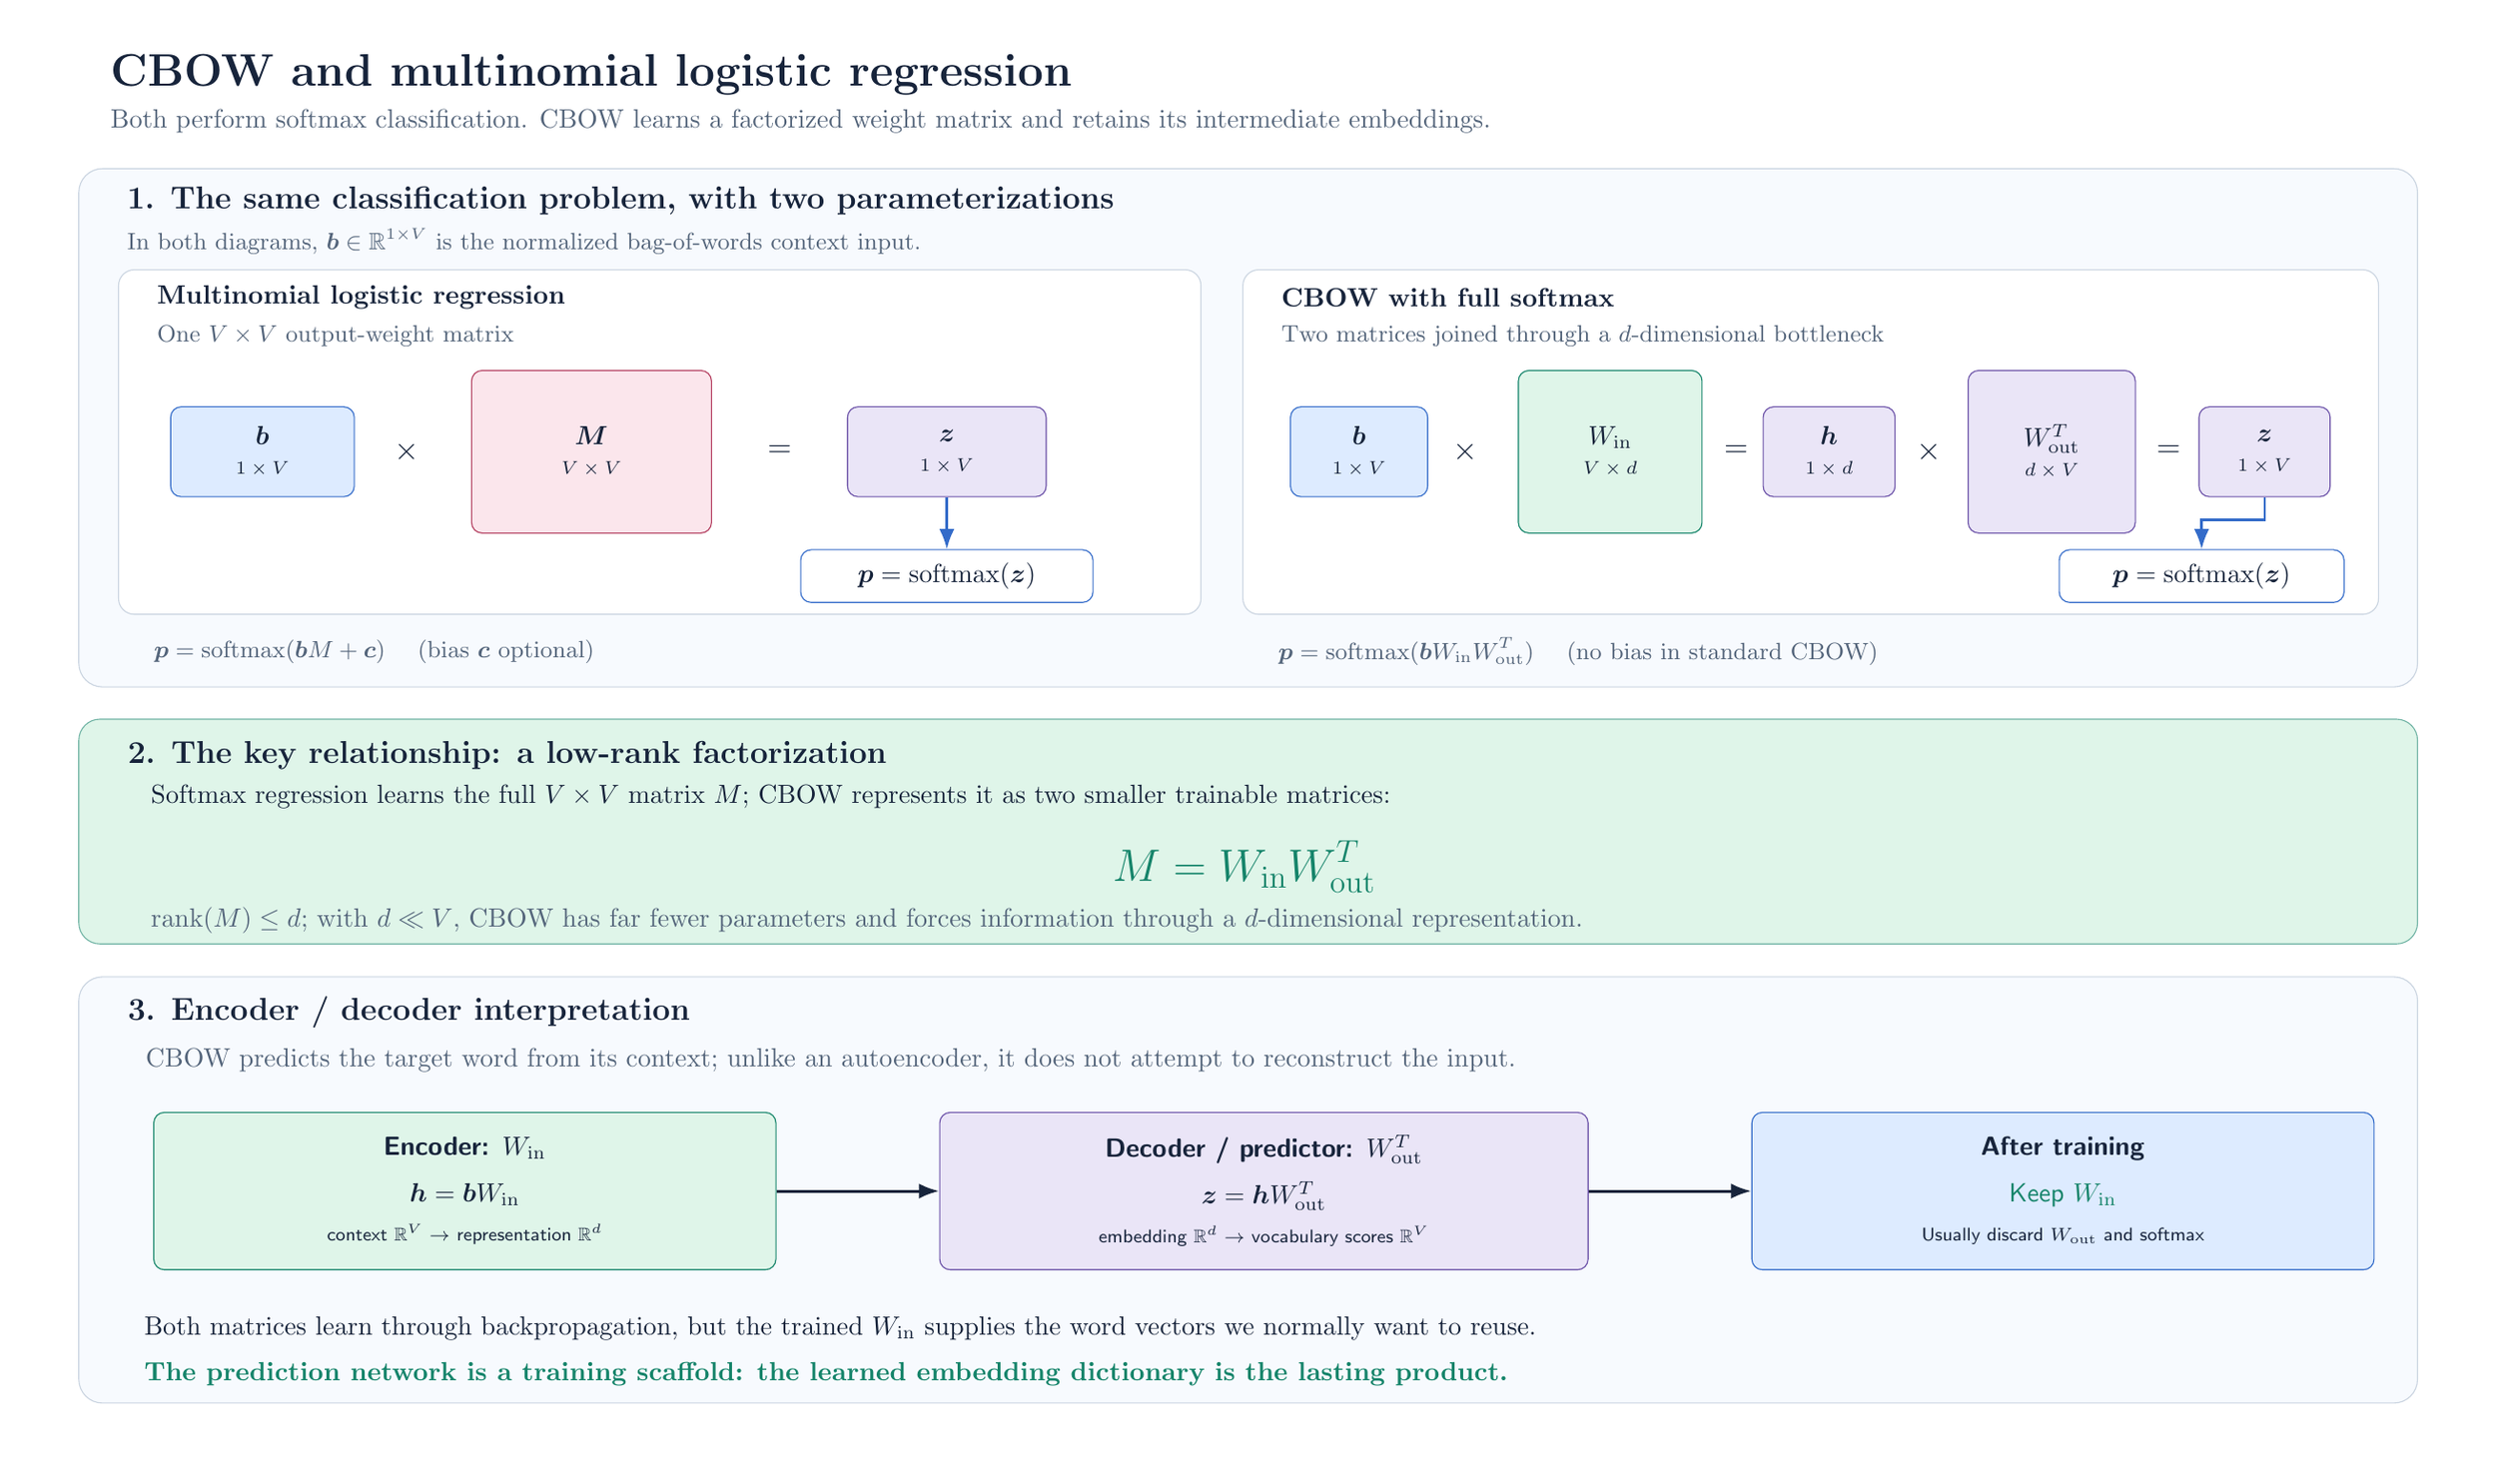
\begin{tikzpicture}[x=1cm,y=1cm,font=\sffamily,text=ink]
\fill[white] (0,0) rectangle (32.6,19.1);

% Heading
\node[anchor=west,font=\bfseries\LARGE] at (1.0,18.45)
  {CBOW and multinomial logistic regression};
\node[anchor=west,text=muted,font=\normalsize] at (1.0,17.83)
  {Both perform softmax classification. CBOW learns a factorized weight matrix and retains its intermediate embeddings.};

% ==================== Comparison ====================
\filldraw[draw=line,fill=panelbg,rounded corners=9pt]
  (0.7,10.28) rectangle (31.9,17.20);
\node[anchor=west,font=\bfseries\large] at (1.22,16.77)
  {1. The same classification problem, with two parameterizations};
\node[anchor=west,font=\small,text=muted] at (1.22,16.23)
  {In both diagrams, $\boldsymbol b\in\mathbb R^{1\times V}$ is the normalized bag-of-words context input.};

% Separate diagrams in their own panels
\filldraw[fill=white,draw=line,rounded corners=6pt] (1.23,11.25) rectangle (15.67,15.85);
\filldraw[fill=white,draw=line,rounded corners=6pt] (16.23,11.25) rectangle (31.38,15.85);
\node[anchor=west,font=\bfseries\normalsize] at (1.62,15.48)
  {Multinomial logistic regression};
\node[anchor=west,font=\small,text=muted] at (1.62,14.96)
  {One $V\times V$ output-weight matrix};
\node[anchor=west,font=\bfseries\normalsize] at (16.62,15.48)
  {CBOW with full softmax};
\node[anchor=west,font=\small,text=muted] at (16.62,14.96)
  {Two matrices joined through a $d$-dimensional bottleneck};

% LEFT diagram - well separated: b x M = z, then softmax
\node[box,draw=blue,fill=selectB,minimum width=2.45cm,minimum height=1.20cm] (lgB) at (3.15,13.42)
  {$\boldsymbol b$\\[-0.3mm]\scriptsize $1\times V$};
\node[font=\large] at (5.08,13.42) {$\times$};
\node[box,draw=pink,fill=palepink,minimum width=3.20cm,minimum height=2.17cm] (lgM) at (7.54,13.42)
  {$\boldsymbol M$\\[-0.3mm]\scriptsize $V\times V$};
\node[font=\large] at (10.05,13.42) {$=$};
\node[box,draw=violet,fill=paleviolet,minimum width=2.65cm,minimum height=1.20cm] (lgZ) at (12.28,13.42)
  {$\boldsymbol z$\\[-0.3mm]\scriptsize $1\times V$};
\node[box,draw=blue,fill=white,minimum width=3.90cm,minimum height=0.64cm] (lgP) at (12.28,11.76)
  {$\boldsymbol p=\operatorname{softmax}(\boldsymbol z)$};
\draw[->,draw=blue,line width=1.0pt] (lgZ.south) -- (lgP.north);

% RIGHT diagram - b x Win = h x Wout^T = z, then softmax
\node[box,draw=blue,fill=selectB,minimum width=1.83cm,minimum height=1.20cm] (cbB) at (17.78,13.42)
  {$\boldsymbol b$\\[-0.3mm]\scriptsize $1\times V$};
\node[font=\large] at (19.20,13.42) {$\times$};
\node[box,draw=teal,fill=selectA,minimum width=2.45cm,minimum height=2.17cm] (cbWin) at (21.13,13.42)
  {$W_{\rm in}$\\[-0.3mm]\scriptsize $V\times d$};
\node[font=\large] at (22.81,13.42) {$=$};
\node[box,draw=violet,fill=paleviolet,minimum width=1.76cm,minimum height=1.20cm] (cbH) at (24.05,13.42)
  {$\boldsymbol h$\\[-0.3mm]\scriptsize $1\times d$};
\node[font=\large] at (25.38,13.42) {$\times$};
\node[box,draw=violet,fill=paleviolet,minimum width=2.23cm,minimum height=2.17cm] (cbWout) at (27.02,13.42)
  {$W_{\rm out}^{T}$\\[-0.3mm]\scriptsize $d\times V$};
\node[font=\large] at (28.58,13.42) {$=$};
\node[box,draw=violet,fill=paleviolet,minimum width=1.75cm,minimum height=1.20cm] (cbZ) at (29.86,13.42)
  {$\boldsymbol z$\\[-0.3mm]\scriptsize $1\times V$};
\node[box,draw=blue,fill=white,minimum width=3.80cm,minimum height=0.64cm] (cbP) at (29.02,11.76)
  {$\boldsymbol p=\operatorname{softmax}(\boldsymbol z)$};
\draw[->,draw=blue,line width=1.0pt]
  (cbZ.south) -- ++(0,-0.30) -| (cbP.north);

% Equations under the separate comparison diagrams, inside outer panel
\node[anchor=west,font=\small,text=muted] at (1.58,10.75)
  {$\displaystyle \boldsymbol p=\operatorname{softmax}(\boldsymbol bM+\boldsymbol c)$ \quad (bias $\boldsymbol c$ optional)};
\node[anchor=west,font=\small,text=muted] at (16.58,10.75)
  {$\displaystyle \boldsymbol p=\operatorname{softmax}(\boldsymbol bW_{\rm in}W_{\rm out}^{T})$ \quad (no bias in standard CBOW)};

% ==================== Factorization ====================
\filldraw[draw=teal!60,fill=selectA,rounded corners=8pt]
  (0.7,6.85) rectangle (31.9,9.85);
\node[anchor=west,font=\bfseries\large] at (1.23,9.37)
  {2. The key relationship: a low-rank factorization};
\node[anchor=west,font=\normalsize] at (1.54,8.82)
  {Softmax regression learns the full $V\times V$ matrix $M$; CBOW represents it as two smaller trainable matrices:};
\node[font=\LARGE,text=teal] at (16.25,7.88)
  {$\displaystyle M=W_{\rm in}W_{\rm out}^{T}$};
\node[anchor=west,font=\normalsize,text=muted] at (1.54,7.16)
  {$\operatorname{rank}(M)\le d$; with $d\ll V$, CBOW has far fewer parameters and forces information through a $d$-dimensional representation.};

% ==================== Encoder / Decoder ====================
\filldraw[draw=line,fill=panelbg,rounded corners=9pt]
  (0.7,0.72) rectangle (31.9,6.41);
\node[anchor=west,font=\bfseries\large] at (1.23,5.93)
  {3. Encoder / decoder interpretation};
\node[anchor=west,font=\normalsize,text=muted] at (1.47,5.30)
  {CBOW predicts the target word from its context; unlike an autoencoder, it does not attempt to reconstruct the input.};

% Three generously spaced conceptual stages
\node[box,draw=teal,fill=selectA,minimum width=8.30cm,minimum height=2.10cm] (enc) at (5.85,3.55)
  {\textbf{Encoder: $W_{\rm in}$}\\[2mm]
   $\boldsymbol h=\boldsymbol bW_{\rm in}$\\[1mm]
   {\scriptsize context $\mathbb R^V\rightarrow$ representation $\mathbb R^d$}};
\node[box,draw=violet,fill=paleviolet,minimum width=8.65cm,minimum height=2.10cm] (dec) at (16.51,3.55)
  {\textbf{Decoder / predictor: $W_{\rm out}^{T}$}\\[2mm]
   $\boldsymbol z=\boldsymbol hW_{\rm out}^{T}$\\[1mm]
   {\scriptsize embedding $\mathbb R^d\rightarrow$ vocabulary scores $\mathbb R^V$}};
\node[box,draw=blue,fill=selectB,minimum width=8.30cm,minimum height=2.10cm] (after) at (27.17,3.55)
  {\textbf{After training}\\[2mm]
   \textcolor{teal}{Keep $W_{\rm in}$}\\[1mm]
   {\scriptsize Usually discard $W_{\rm out}$ and softmax}};
\draw[flow] (enc.east) -- (dec.west);
\draw[flow] (dec.east) -- (after.west);

\node[anchor=west,font=\normalsize] at (1.45,1.72)
  {Both matrices learn through backpropagation, but the trained $W_{\rm in}$ supplies the word vectors we normally want to reuse.};
\node[anchor=west,font=\bfseries\normalsize,text=teal] at (1.45,1.10)
  {The prediction network is a training scaffold: the learned embedding dictionary is the lasting product.};
\end{tikzpicture}



% ============ PAGE 6: SKIP-GRAM, THE MIRROR IMAGE OF CBOW ============
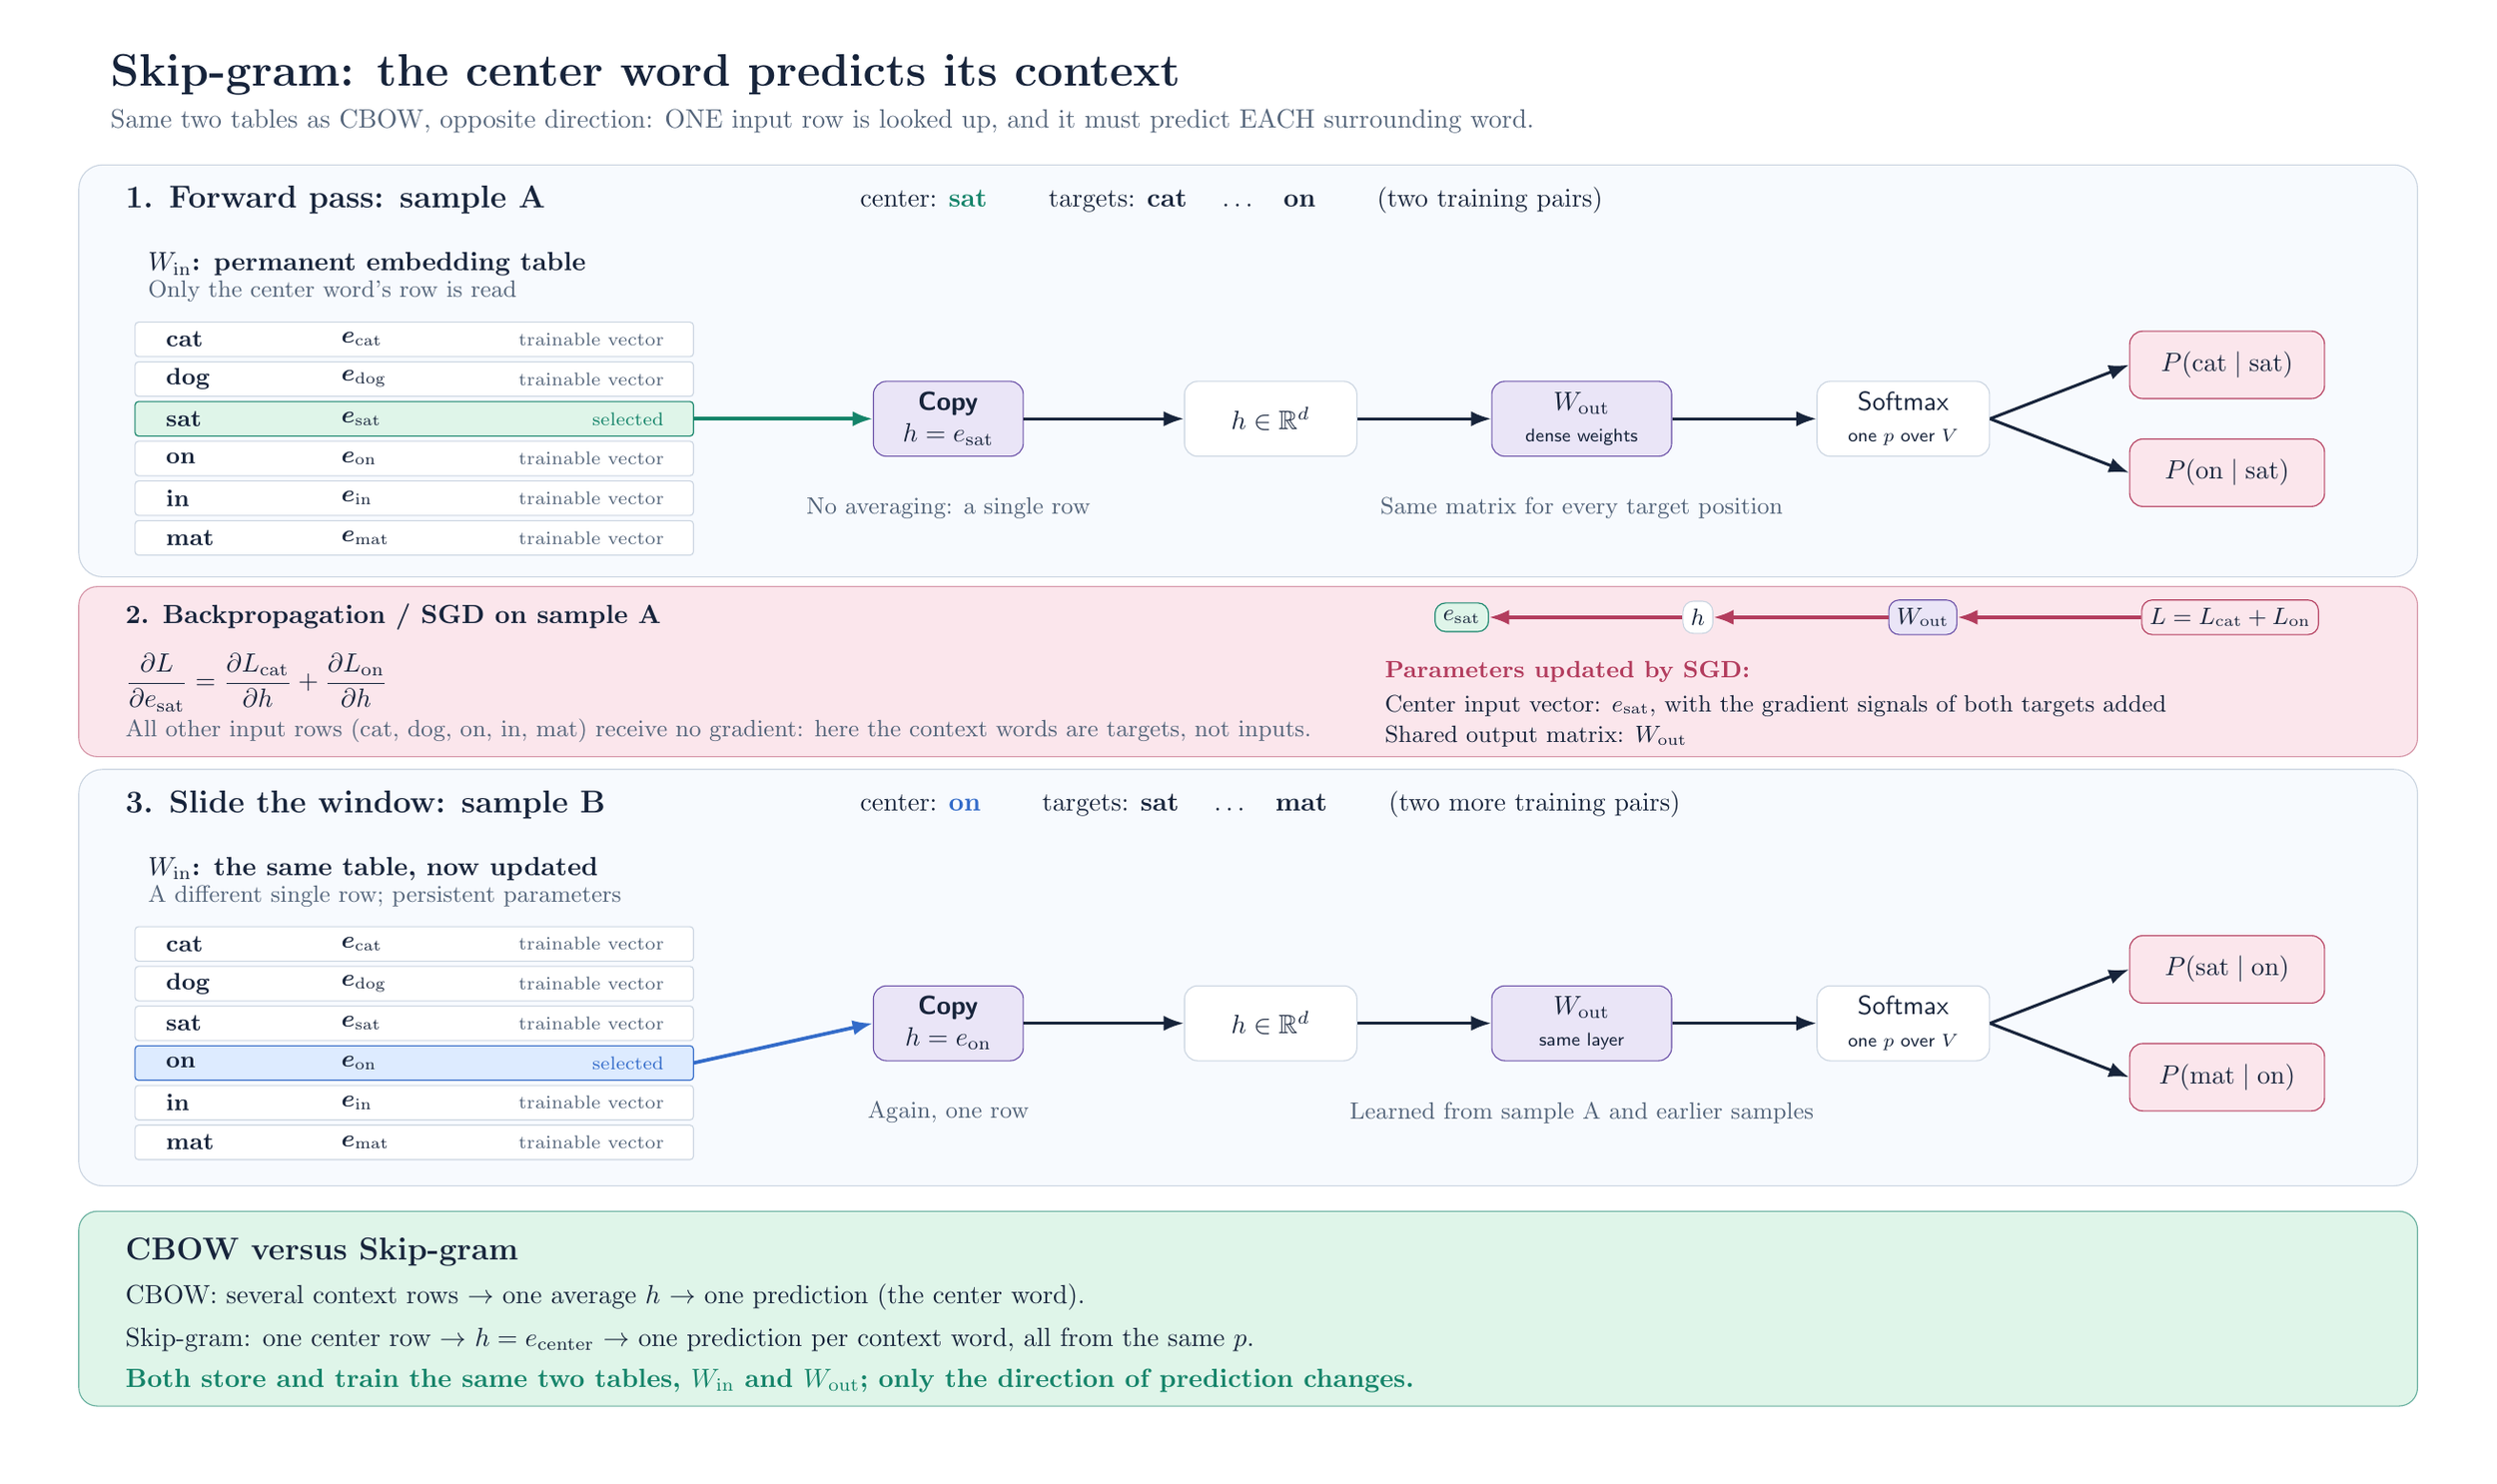
\begin{tikzpicture}[x=1cm,y=1cm,font=\sffamily,text=ink]
\fill[white] (0,0) rectangle (32.6,19.1);
\node[anchor=west,font=\bfseries\LARGE] at (1,18.45)
  {Skip-gram: the center word predicts its context};
\node[anchor=west,text=muted,font=\normalsize] at (1,17.83)
  {Same two tables as CBOW, opposite direction: ONE input row is looked up, and it must predict EACH surrounding word.};

% --- Panel A ---
\filldraw[fill=panelbg,draw=line,rounded corners=9pt] (0.7,11.75) rectangle (31.9,17.25);
\node[anchor=west,font=\bfseries\large] at (1.2,16.78) {1. Forward pass: sample A};
\node[anchor=west,font=\normalsize] at (11.0,16.78)
  {center: \textcolor{teal}{\textbf{sat}} \qquad targets: \textbf{cat} \quad \ldots \quad \textbf{on} \qquad (two training pairs)};
\node[anchor=west,font=\bfseries\normalsize] at (1.5,15.92)
  {$W_{\mathrm{in}}$: permanent embedding table};
\node[anchor=west,text=muted,font=\small] at (1.5,15.56) {Only the center word's row is read};

\foreach \word/\symbol/\y in {
  cat/cat/14.92,dog/dog/14.39,sat/sat/13.86,on/on/13.33,in/in/12.80,mat/mat/12.27}
{
  \filldraw[fill=white,draw=line,rounded corners=1.3pt] (1.45,\y-0.23) rectangle (8.90,\y+0.23);
  \node[anchor=west,font=\small\bfseries] at (1.74,\y) {\word};
  \node[anchor=west,font=\small] at (4.08,\y) {$\boldsymbol e_{\mathrm{\symbol}}$};
  \node[anchor=east,text=muted,font=\scriptsize] at (8.63,\y) {trainable vector};
}
\filldraw[fill=selectA,draw=teal,rounded corners=1.3pt] (1.45,13.63) rectangle (8.9,14.09);
\node[anchor=west,font=\small\bfseries] at (1.74,13.86) {sat};
\node[anchor=west,font=\small] at (4.08,13.86) {$\boldsymbol e_{\mathrm{sat}}$};
\node[anchor=east,font=\scriptsize,text=teal] at (8.63,13.86) {selected};

\node[avg] (sgCopyA) at (12.3,13.86) {\textbf{Copy}\\$h=e_{\rm sat}$};
\node[stage] (sgHA) at (16.6,13.86) {$h\in\mathbb{R}^d$};
\node[classifier] (sgOutA) at (20.75,13.86) {$W_{\rm out}$\\\scriptsize dense weights};
\node[stage] (sgSoftA) at (25.04,13.86) {Softmax\\\scriptsize one $p$ over $V$};
\node[target,minimum height=0.9cm] (sgTA1) at (29.36,14.58) {$P(\mathrm{cat}\mid\mathrm{sat})$};
\node[target,minimum height=0.9cm] (sgTA2) at (29.36,13.14) {$P(\mathrm{on}\mid\mathrm{sat})$};
\draw[linkA] (8.9,13.86) -- (sgCopyA.west);
\draw[flow] (sgCopyA.east) -- (sgHA.west);
\draw[flow] (sgHA.east) -- (sgOutA.west);
\draw[flow] (sgOutA.east) -- (sgSoftA.west);
\draw[flow] (sgSoftA.east) -- (sgTA1.west);
\draw[flow] (sgSoftA.east) -- (sgTA2.west);
\node[anchor=north,font=\small,text=muted] at (12.3,12.93) {No averaging: a single row};
\node[anchor=north,font=\small,text=muted] at (20.75,12.93) {Same matrix for every target position};

% --- Gradient strip ---
\filldraw[draw=pink!55,fill=palepink,rounded corners=7pt]
  (0.7,9.35) rectangle (31.9,11.62);
\node[anchor=west,font=\bfseries\normalsize] at (1.2,11.22)
  {2. Backpropagation / SGD on sample A};

\node[box,draw=teal,fill=selectA,inner sep=3pt,font=\small] (sgGradEmb) at (19.15,11.21)
  {$e_{\rm sat}$};
\node[box,inner sep=3pt,font=\small] (sgGradH) at (22.30,11.21) {$h$};
\node[box,draw=violet,fill=paleviolet,inner sep=3pt,font=\small] (sgGradW) at (25.30,11.21)
  {$W_{\rm out}$};
\node[box,draw=pink,fill=palepink,inner sep=3pt,font=\small] (sgGradL) at (29.40,11.21)
  {$L=L_{\rm cat}+L_{\rm on}$};
\draw[reverse] (sgGradL.west) -- (sgGradW.east);
\draw[reverse] (sgGradW.west) -- (sgGradH.east);
\draw[reverse] (sgGradH.west) -- (sgGradEmb.east);

\node[anchor=north west,font=\normalsize] at (1.2,10.85)
  {$\displaystyle \frac{\partial L}{\partial e_{\rm sat}}
                =\frac{\partial L_{\rm cat}}{\partial h}
                +\frac{\partial L_{\rm on}}{\partial h}$};
\node[anchor=west,text=muted,font=\small] at (1.2,9.69)
  {All other input rows (cat, dog, on, in, mat) receive no gradient: here the context words are targets, not inputs.};

\node[anchor=west,font=\bfseries\small,text=pink] at (18.0,10.48)
  {Parameters updated by SGD:};
\node[anchor=west,font=\small] at (18.0,10.03)
  {Center input vector: $e_{\rm sat}$, with the gradient signals of both targets added};
\node[anchor=west,font=\small] at (18.0,9.62)
  {Shared output matrix: $W_{\rm out}$};

% --- Panel B ---
\filldraw[fill=panelbg,draw=line,rounded corners=9pt] (0.7,3.62) rectangle (31.9,9.18);
\node[anchor=west,font=\bfseries\large] at (1.2,8.71) {3. Slide the window: sample B};
\node[anchor=west,font=\normalsize] at (11.0,8.71)
  {center: \textcolor{blue}{\textbf{on}} \qquad targets: \textbf{sat} \quad \ldots \quad \textbf{mat} \qquad (two more training pairs)};
\node[anchor=west,font=\bfseries\normalsize] at (1.5,7.85)
  {$W_{\mathrm{in}}$: the same table, now updated};
\node[anchor=west,text=muted,font=\small] at (1.5,7.49) {A different single row; persistent parameters};

\foreach \word/\symbol/\y in {
  cat/cat/6.85,dog/dog/6.32,sat/sat/5.79,on/on/5.26,in/in/4.73,mat/mat/4.20}
{
  \filldraw[fill=white,draw=line,rounded corners=1.3pt] (1.45,\y-0.23) rectangle (8.90,\y+0.23);
  \node[anchor=west,font=\small\bfseries] at (1.74,\y) {\word};
  \node[anchor=west,font=\small] at (4.08,\y) {$\boldsymbol e_{\mathrm{\symbol}}$};
  \node[anchor=east,text=muted,font=\scriptsize] at (8.63,\y) {trainable vector};
}
\filldraw[fill=selectB,draw=blue,rounded corners=1.3pt] (1.45,5.03) rectangle (8.9,5.49);
\node[anchor=west,font=\small\bfseries] at (1.74,5.26) {on};
\node[anchor=west,font=\small] at (4.08,5.26) {$\boldsymbol e_{\mathrm{on}}$};
\node[anchor=east,font=\scriptsize,text=blue] at (8.63,5.26) {selected};

\node[avg] (sgCopyB) at (12.3,5.79) {\textbf{Copy}\\$h=e_{\rm on}$};
\node[stage] (sgHB) at (16.6,5.79) {$h\in\mathbb{R}^d$};
\node[classifier] (sgOutB) at (20.75,5.79) {$W_{\rm out}$\\\scriptsize same layer};
\node[stage] (sgSoftB) at (25.04,5.79) {Softmax\\\scriptsize one $p$ over $V$};
\node[target,minimum height=0.9cm] (sgTB1) at (29.36,6.51) {$P(\mathrm{sat}\mid\mathrm{on})$};
\node[target,minimum height=0.9cm] (sgTB2) at (29.36,5.07) {$P(\mathrm{mat}\mid\mathrm{on})$};
\draw[linkB] (8.9,5.26) -- (sgCopyB.west);
\draw[flow] (sgCopyB.east) -- (sgHB.west);
\draw[flow] (sgHB.east) -- (sgOutB.west);
\draw[flow] (sgOutB.east) -- (sgSoftB.west);
\draw[flow] (sgSoftB.east) -- (sgTB1.west);
\draw[flow] (sgSoftB.east) -- (sgTB2.west);
\node[anchor=north,font=\small,text=muted] at (12.3,4.86) {Again, one row};
\node[anchor=north,font=\small,text=muted] at (20.75,4.86) {Learned from sample A and earlier samples};

% Takeaway strip
\filldraw[draw=teal!65,fill=selectA,rounded corners=7pt] (0.7,0.68) rectangle (31.9,3.28);
\node[anchor=west,font=\bfseries\large] at (1.2,2.73) {CBOW versus Skip-gram};
\node[anchor=west,font=\normalsize] at (1.2,2.13)
  {CBOW: several context rows $\rightarrow$ one average $h$ $\rightarrow$ one prediction (the center word).};
\node[anchor=west,font=\normalsize] at (1.2,1.56)
  {Skip-gram: one center row $\rightarrow$ $h=e_{\rm center}$ $\rightarrow$ one prediction per context word, all from the same $p$.};
\node[anchor=west,font=\bfseries\normalsize,text=teal] at (1.2,1.02)
  {Both store and train the same two tables, $W_{\rm in}$ and $W_{\rm out}$; only the direction of prediction changes.};
\end{tikzpicture}



% ============ PAGE 7: SKIP-GRAM MATRIX FORMULATION, C = 7 ============
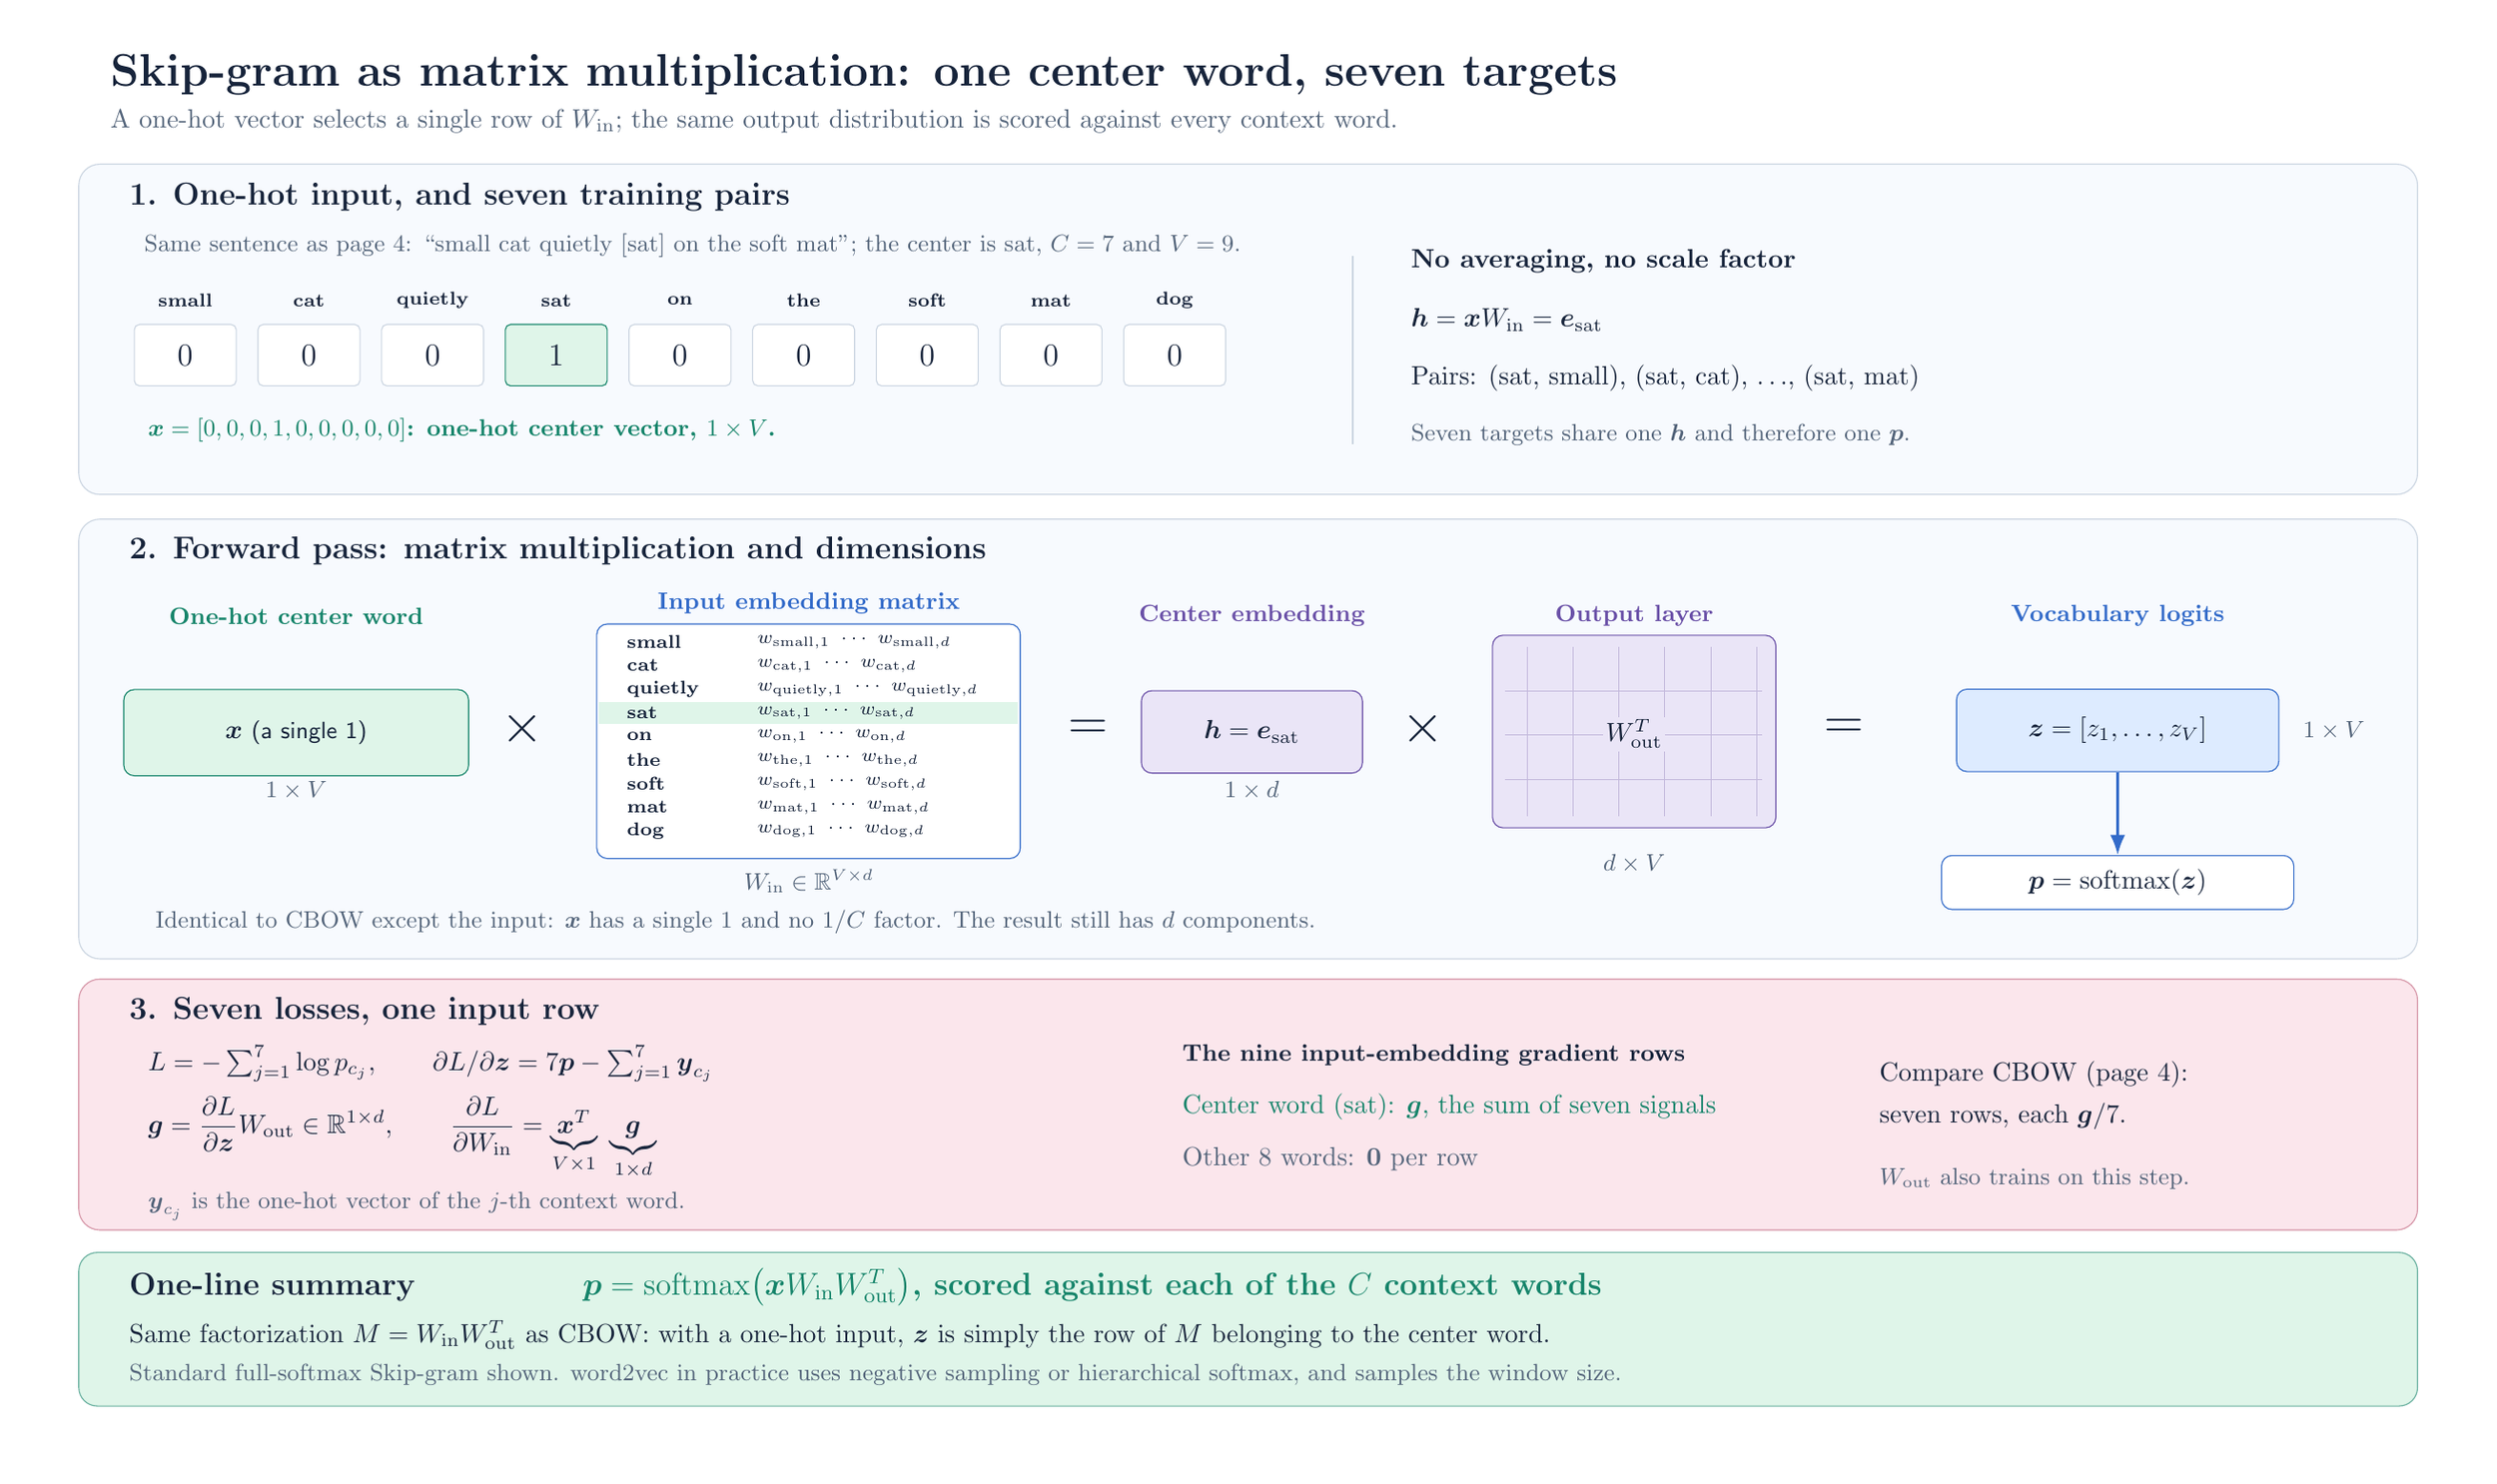
\begin{tikzpicture}[x=1cm,y=1cm,font=\sffamily,text=ink]
\fill[white] (0,0) rectangle (32.6,19.1);
\node[anchor=west,font=\bfseries\LARGE] at (1.0,18.45)
  {Skip-gram as matrix multiplication: one center word, seven targets};
\node[anchor=west,font=\normalsize,text=muted] at (1.0,17.83)
  {A one-hot vector selects a single row of $W_{\rm in}$; the same output distribution is scored against every context word.};

% SECTION 1: ONE-HOT INPUT
\filldraw[draw=line,fill=panelbg,rounded corners=8pt] (0.7,12.85) rectangle (31.9,17.26);
\node[anchor=west,font=\bfseries\large] at (1.25,16.82) {1. One-hot input, and seven training pairs};
\node[anchor=west,font=\small,text=muted] at (1.45,16.17)
  {Same sentence as page 4: ``small cat quietly [sat] on the soft mat''; the center is sat, $C=7$ and $V=9$.};

\foreach \w/\idx/\flag in {small/0/0,cat/1/0,quietly/2/0,sat/3/1,on/4/0,the/5/0,soft/6/0,mat/7/0,dog/8/0}{
  \pgfmathsetmacro{\xx}{2.12+1.65*\idx}
  \node[font=\scriptsize\bfseries] at (\xx,15.44) {\w};
  \ifnum\flag=1
    \filldraw[draw=teal,fill=selectA,rounded corners=2pt] (\xx-0.68,14.30) rectangle (\xx+0.68,15.12);
  \else
    \filldraw[draw=line,fill=white,rounded corners=2pt] (\xx-0.68,14.30) rectangle (\xx+0.68,15.12);
  \fi
  \node[font=\large] at (\xx,14.71) {$\flag$};
}
\node[anchor=west,font=\small\bfseries,text=teal] at (1.50,13.71)
  {$\boldsymbol x=[0,0,0,1,0,0,0,0,0]$: one-hot center vector, $1\times V$.};
\draw[draw=line,line width=.7pt] (17.70,13.52)--(17.70,16.04);
\node[anchor=west,font=\bfseries\normalsize] at (18.35,15.96) {No averaging, no scale factor};
\node[anchor=west,font=\normalsize] at (18.35,15.18)
  {$\displaystyle \boldsymbol h=\boldsymbol xW_{\rm in}=\boldsymbol e_{\rm sat}$};
\node[anchor=west,font=\normalsize] at (18.35,14.40)
  {Pairs: (sat, small), (sat, cat), $\ldots$, (sat, mat)};
\node[anchor=west,font=\small,text=muted] at (18.35,13.64)
  {Seven targets share one $\boldsymbol h$ and therefore one $\boldsymbol p$.};

% SECTION 2: MAIN MATRIX PIPELINE
\filldraw[draw=line,fill=panelbg,rounded corners=8pt] (0.7,6.65) rectangle (31.9,12.52);
\node[anchor=west,font=\bfseries\large] at (1.25,12.09) {2. Forward pass: matrix multiplication and dimensions};
\node[font=\bfseries\small,text=teal] at (3.60,11.23) {One-hot center word};
\node[box,draw=teal,fill=selectA,minimum width=4.6cm,minimum height=1.15cm] at (3.60,9.67)
  {$\boldsymbol x$ \small(a single 1)};
\node[font=\small,text=muted] at (3.60,8.90) {$1\times V$};
\node[font=\huge] at (6.62,9.72) {$\times$};
\node[font=\bfseries\small,text=blue] at (10.44,11.39) {Input embedding matrix};
\filldraw[draw=blue,fill=white,rounded corners=4pt] (7.61,7.99) rectangle (13.26,11.12);
\foreach \w/\idx/\flag in {small/0/0,cat/1/0,quietly/2/0,sat/3/1,on/4/0,the/5/0,soft/6/0,mat/7/0,dog/8/0}{
  \pgfmathsetmacro{\yy}{10.88-0.315*\idx}
  \ifnum\flag=1
    \fill[selectA] (7.64,\yy-0.145) rectangle (13.22,\yy+0.145);
  \fi
  \node[anchor=west,font=\scriptsize\bfseries] at (7.89,\yy) {\w};
  \node[anchor=west,font=\scriptsize] at (9.63,\yy) {$w_{\mathrm{\w},1}\ \cdots\ w_{\mathrm{\w},d}$};
}
\node[font=\small,text=muted] at (10.44,7.69) {$W_{\rm in}\in\mathbb R^{V\times d}$};
\node[font=\huge] at (14.17,9.71) {$=$};
\node[font=\bfseries\small,text=violet] at (16.35,11.23) {Center embedding};
\node[box,draw=violet,fill=paleviolet,minimum width=2.95cm,minimum height=1.1cm] at (16.35,9.68)
  {$\boldsymbol h=\boldsymbol e_{\rm sat}$};
\node[font=\small,text=muted] at (16.35,8.90) {$1\times d$};
\node[font=\huge] at (18.63,9.72) {$\times$};
\node[font=\bfseries\small,text=violet] at (21.45,11.23) {Output layer};
\filldraw[draw=violet,fill=paleviolet,rounded corners=4pt] (19.56,8.40) rectangle (23.34,10.97);
\foreach \x in {20.03,20.64,21.25,21.86,22.47,23.08}{
  \draw[draw=violet!40,line width=.35pt] (\x,8.55)--(\x,10.82);
}
\foreach \y in {9.05,9.64,10.23}{
  \draw[draw=violet!40,line width=.35pt] (19.73,\y)--(23.15,\y);
}
\node[fill=paleviolet,inner sep=1pt,font=\bfseries\normalsize] at (21.45,9.65) {$W_{\rm out}^{T}$};
\node[font=\small,text=muted] at (21.45,7.92) {$d\times V$};
\node[font=\huge] at (24.25,9.72) {$=$};
\node[font=\bfseries\small,text=blue] at (27.90,11.23) {Vocabulary logits};
\node[box,draw=blue,fill=selectB,minimum width=4.3cm,minimum height=1.1cm] (sgmz) at (27.90,9.70)
  {$\boldsymbol z=[z_1,\ldots,z_V]$};
\node[font=\small,text=muted,anchor=west] at (30.25,9.70) {$1\times V$};
\node[box,draw=blue,fill=white,minimum width=4.7cm,minimum height=0.72cm]
  (sgprob) at (27.90,7.67) {$\boldsymbol p=\operatorname{softmax}(\boldsymbol z)$};
\draw[->,draw=blue,line width=1pt] (sgmz.south) -- (sgprob.north);
\node[anchor=west,font=\small,text=muted] at (1.60,7.14)
  {Identical to CBOW except the input: $\boldsymbol x$ has a single 1 and no $1/C$ factor. The result still has $d$ components.};

% SECTION 3: LOSS AND GRADIENT
\filldraw[draw=pink!55,fill=palepink,rounded corners=8pt] (0.7,3.03) rectangle (31.9,6.38);
\node[anchor=west,font=\bfseries\large] at (1.25,5.95) {3. Seven losses, one input row};
\node[anchor=west,font=\normalsize] at (1.50,5.25)
  {$L=-\sum_{j=1}^{7}\log p_{c_j}, \qquad
    \partial L/\partial\boldsymbol z=7\boldsymbol p-\sum_{j=1}^{7}\boldsymbol y_{c_j}$};
\node[anchor=west,font=\normalsize] at (1.50,4.25)
  {$\displaystyle \boldsymbol g=\frac{\partial L}{\partial\boldsymbol z}W_{\rm out}\in\mathbb R^{1\times d},\qquad
    \frac{\partial L}{\partial W_{\rm in}}=\underbrace{\boldsymbol x^T}_{V\times1}\;\underbrace{\boldsymbol g}_{1\times d}$};
\node[anchor=west,font=\small,text=muted] at (1.50,3.35)
  {$\boldsymbol y_{c_j}$ is the one-hot vector of the $j$-th context word.};
\node[anchor=west,font=\bfseries\small] at (15.30,5.36) {The nine input-embedding gradient rows};
\node[anchor=west,font=\normalsize,text=teal] at (15.30,4.68)
  {Center word (sat): $\boldsymbol g$, the sum of seven signals};
\node[anchor=west,font=\normalsize,text=muted] at (15.30,3.97)
  {Other 8 words: $\boldsymbol 0$ per row};
\node[anchor=west,font=\normalsize] at (24.60,5.10) {Compare CBOW (page 4):};
\node[anchor=west,font=\normalsize] at (24.60,4.55) {seven rows, each $\boldsymbol g/7$.};
\node[anchor=west,font=\small,text=muted] at (24.60,3.71) {$W_{\rm out}$ also trains on this step.};

% BOTTOM
\filldraw[draw=teal!65,fill=selectA,rounded corners=7pt] (0.7,0.68) rectangle (31.9,2.73);
\node[anchor=west,font=\bfseries\large] at (1.25,2.27) {One-line summary};
\node[anchor=west,font=\large\bfseries,text=teal] at (7.3,2.27)
  {$\boldsymbol p=\operatorname{softmax}\!\left(\boldsymbol xW_{\rm in}W_{\rm out}^{T}\right)$, scored against each of the $C$ context words};
\node[anchor=west,font=\normalsize] at (1.25,1.63)
  {Same factorization $M=W_{\rm in}W_{\rm out}^T$ as CBOW: with a one-hot input, $\boldsymbol z$ is simply the row of $M$ belonging to the center word.};
\node[anchor=west,font=\small,text=muted] at (1.25,1.10)
  {Standard full-softmax Skip-gram shown. word2vec in practice uses negative sampling or hierarchical softmax, and samples the window size.};
\end{tikzpicture}



% ============ PAGE 8: CBOW VS SKIP-GRAM SIDE BY SIDE ============
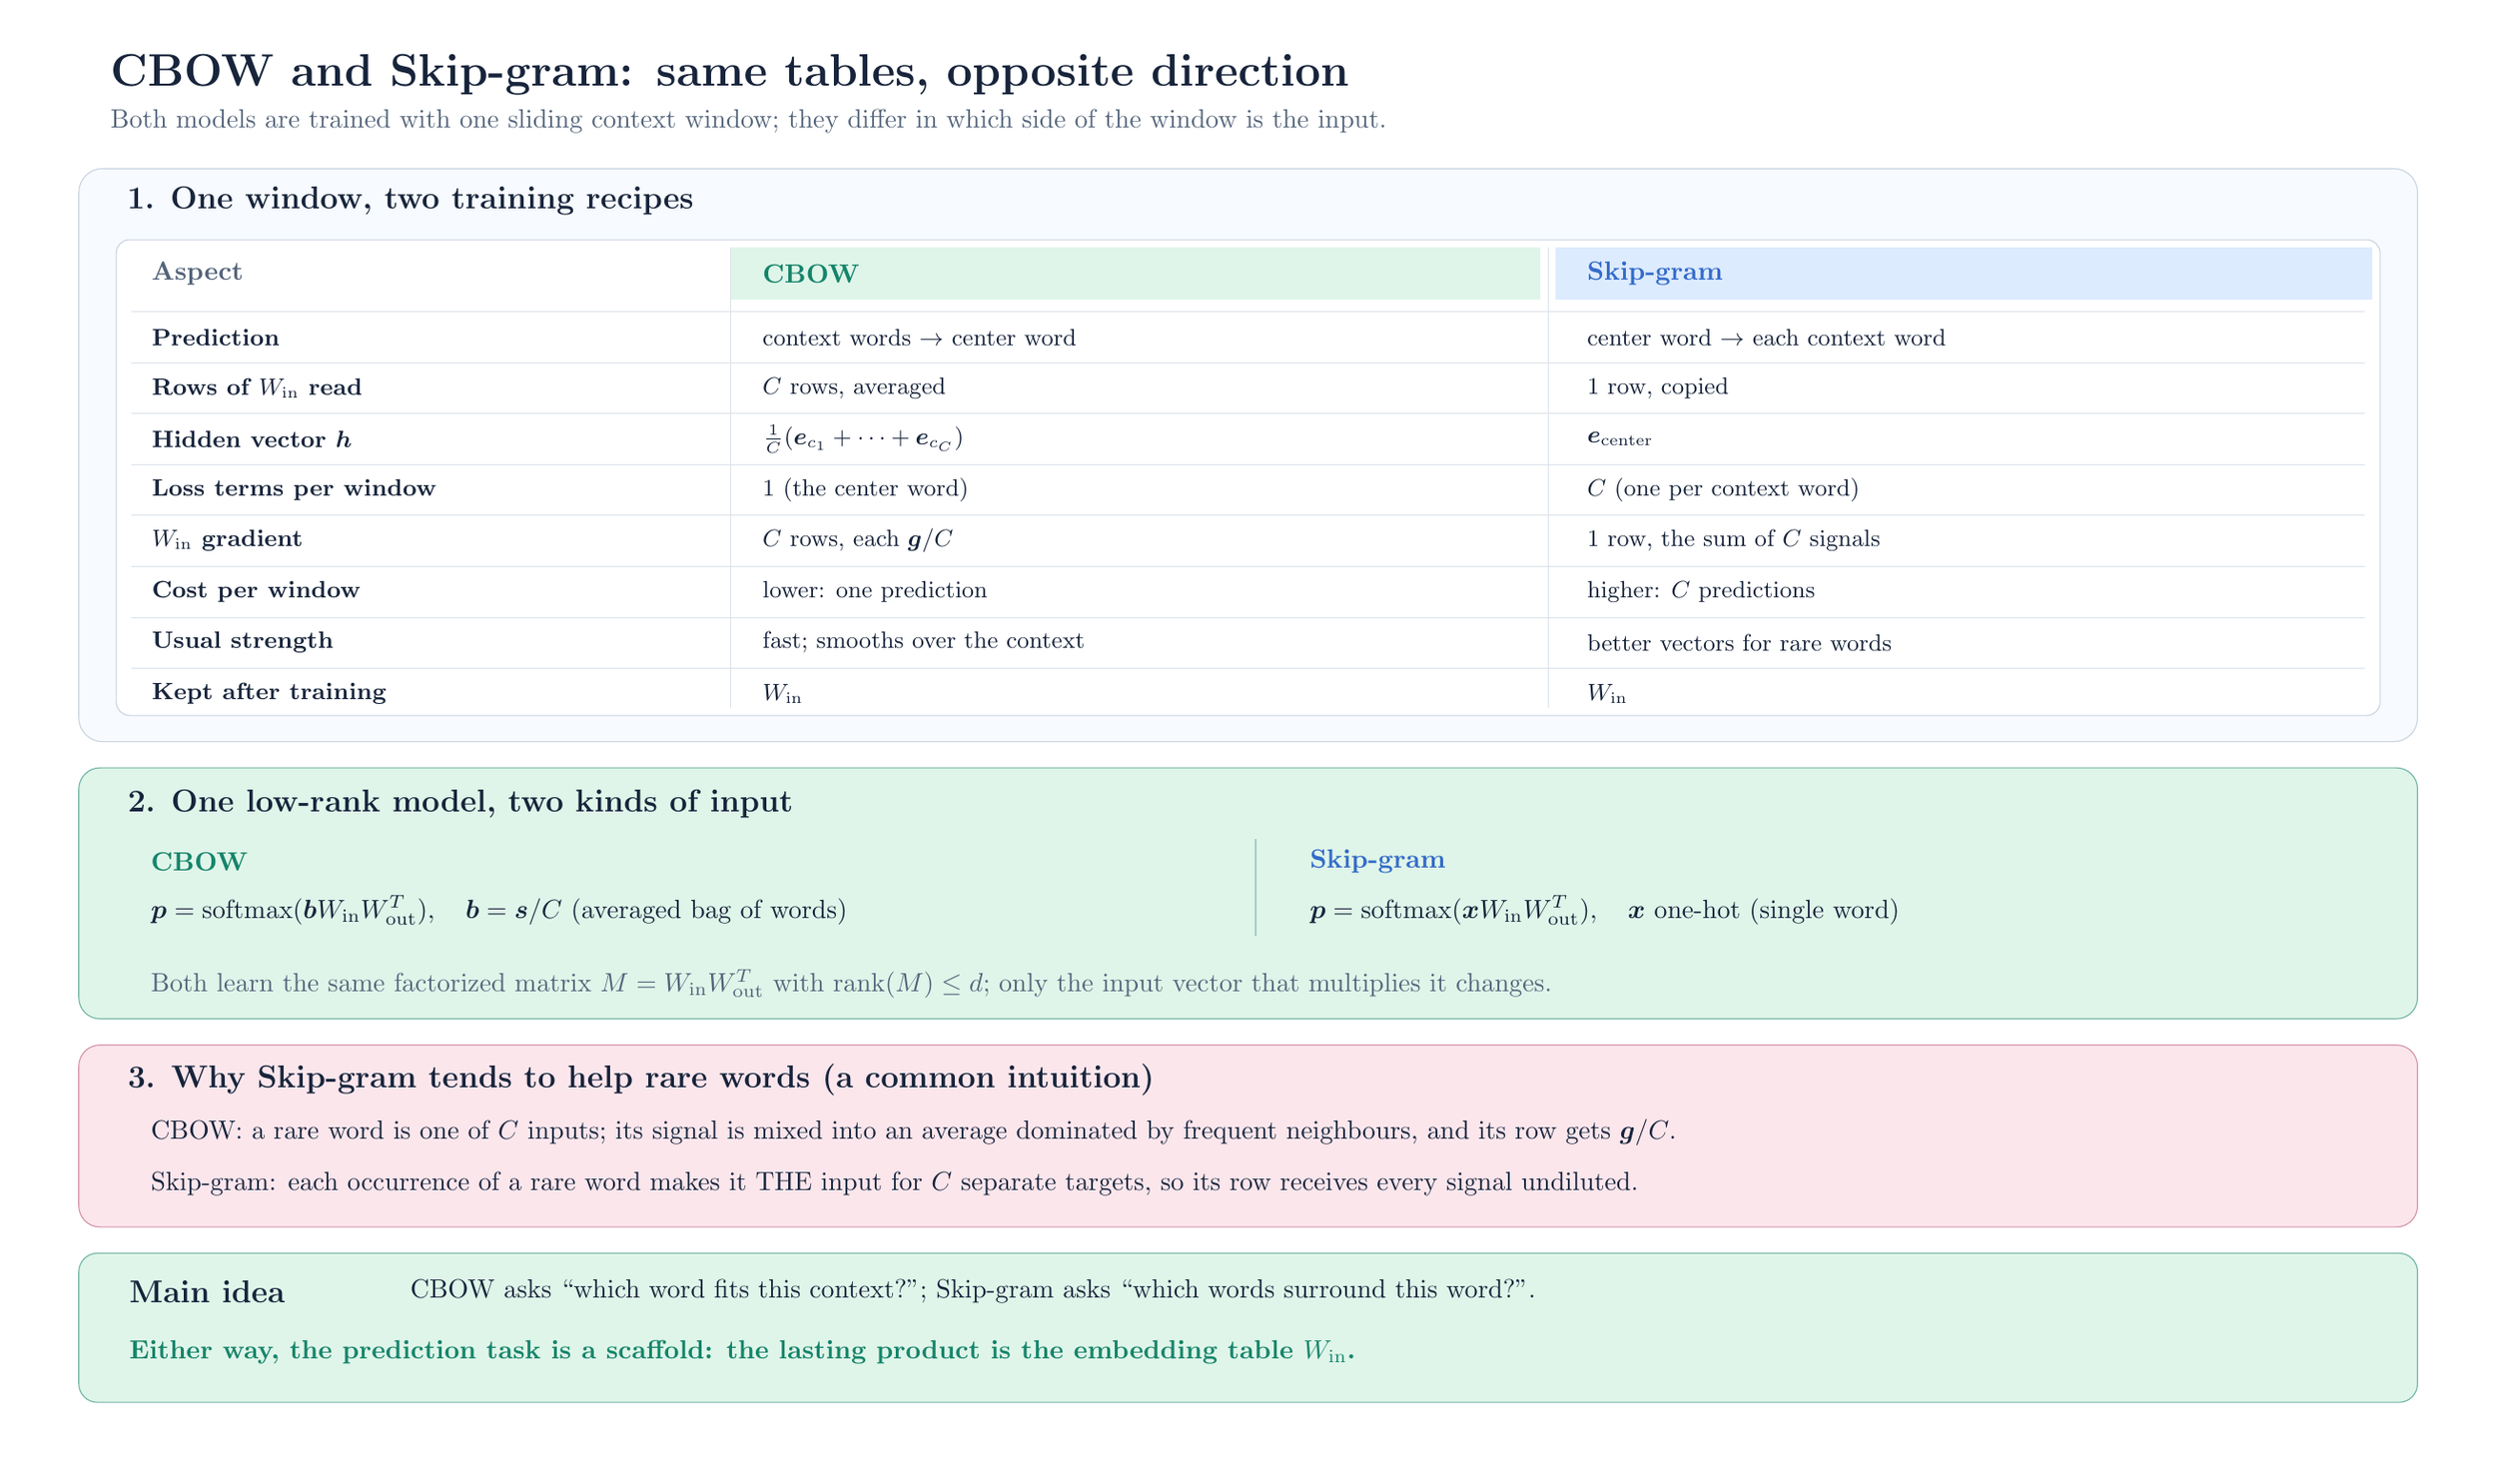
\begin{tikzpicture}[x=1cm,y=1cm,font=\sffamily,text=ink]
\fill[white] (0,0) rectangle (32.6,19.1);
\node[anchor=west,font=\bfseries\LARGE] at (1.0,18.45)
  {CBOW and Skip-gram: same tables, opposite direction};
\node[anchor=west,font=\normalsize,text=muted] at (1.0,17.83)
  {Both models are trained with one sliding context window; they differ in which side of the window is the input.};

% SECTION 1: COMPARISON TABLE
\filldraw[draw=line,fill=panelbg,rounded corners=9pt] (0.7,9.55) rectangle (31.9,17.20);
\node[anchor=west,font=\bfseries\large] at (1.22,16.77) {1. One window, two training recipes};
\filldraw[fill=white,draw=line,rounded corners=5pt] (1.20,9.90) rectangle (31.40,16.25);
\fill[selectA] (9.40,15.45) rectangle (20.20,16.15);
\fill[selectB] (20.40,15.45) rectangle (31.30,16.15);
\node[anchor=west,font=\bfseries\normalsize,text=muted] at (1.55,15.80) {Aspect};
\node[anchor=west,font=\bfseries\normalsize,text=teal] at (9.70,15.80) {CBOW};
\node[anchor=west,font=\bfseries\normalsize,text=blue] at (20.70,15.80) {Skip-gram};
\foreach \aspect/\cbow/\sg [count=\i from 0] in {
  {Prediction}/{context words $\rightarrow$ center word}/{center word $\rightarrow$ each context word},
  {Rows of $W_{\rm in}$ read}/{$C$ rows, averaged}/{1 row, copied},
  {Hidden vector $\boldsymbol h$}/{$\frac1C(\boldsymbol e_{c_1}+\cdots+\boldsymbol e_{c_C})$}/{$\boldsymbol e_{\rm center}$},
  {Loss terms per window}/{1 (the center word)}/{$C$ (one per context word)},
  {$W_{\rm in}$ gradient}/{$C$ rows, each $\boldsymbol g/C$}/{1 row, the sum of $C$ signals},
  {Cost per window}/{lower: one prediction}/{higher: $C$ predictions},
  {Usual strength}/{fast; smooths over the context}/{better vectors for rare words},
  {Kept after training}/{$W_{\rm in}$}/{$W_{\rm in}$}}
{
  \pgfmathsetmacro{\yy}{14.95-0.68*\i}
  \draw[draw=line!70,line width=.3pt] (1.40,\yy+0.34) -- (31.20,\yy+0.34);
  \node[anchor=west,font=\bfseries\small] at (1.55,\yy) {\aspect};
  \node[anchor=west,font=\small] at (9.70,\yy) {\cbow};
  \node[anchor=west,font=\small] at (20.70,\yy) {\sg};
}
\draw[draw=line!70,line width=.3pt] (9.40,10.00) -- (9.40,16.15);
\draw[draw=line!70,line width=.3pt] (20.30,10.00) -- (20.30,16.15);

% SECTION 2: SAME LOW-RANK MODEL
\filldraw[draw=teal!60,fill=selectA,rounded corners=8pt] (0.7,5.85) rectangle (31.9,9.20);
\node[anchor=west,font=\bfseries\large] at (1.23,8.72)
  {2. One low-rank model, two kinds of input};
\node[anchor=west,font=\bfseries\normalsize,text=teal] at (1.54,7.95) {CBOW};
\node[anchor=west,font=\normalsize] at (1.54,7.30)
  {$\displaystyle \boldsymbol p=\operatorname{softmax}(\boldsymbol bW_{\rm in}W_{\rm out}^{T}),\quad \boldsymbol b=\boldsymbol s/C$ (averaged bag of words)};
\node[anchor=west,font=\bfseries\normalsize,text=blue] at (17.00,7.95) {Skip-gram};
\node[anchor=west,font=\normalsize] at (17.00,7.30)
  {$\displaystyle \boldsymbol p=\operatorname{softmax}(\boldsymbol xW_{\rm in}W_{\rm out}^{T}),\quad \boldsymbol x$ one-hot (single word)};
\draw[draw=teal!40,line width=0.7pt] (16.40,6.95) -- (16.40,8.25);
\node[anchor=west,font=\normalsize,text=muted] at (1.54,6.32)
  {Both learn the same factorized matrix $M=W_{\rm in}W_{\rm out}^{T}$ with $\operatorname{rank}(M)\le d$; only the input vector that multiplies it changes.};

% SECTION 3: RARE-WORD INTUITION
\filldraw[draw=pink!55,fill=palepink,rounded corners=8pt] (0.7,3.07) rectangle (31.9,5.50);
\node[anchor=west,font=\bfseries\large] at (1.23,5.03)
  {3. Why Skip-gram tends to help rare words (a common intuition)};
\node[anchor=west,font=\normalsize] at (1.54,4.33)
  {CBOW: a rare word is one of $C$ inputs; its signal is mixed into an average dominated by frequent neighbours, and its row gets $\boldsymbol g/C$.};
\node[anchor=west,font=\normalsize] at (1.54,3.65)
  {Skip-gram: each occurrence of a rare word makes it THE input for $C$ separate targets, so its row receives every signal undiluted.};

% BOTTOM
\filldraw[draw=teal!60,fill=selectA,rounded corners=7pt] (0.7,0.73) rectangle (31.9,2.72);
\node[anchor=west,font=\bfseries\large] at (1.25,2.21) {Main idea};
\node[anchor=west,font=\normalsize] at (5.0,2.21)
  {CBOW asks ``which word fits this context?''; Skip-gram asks ``which words surround this word?''.};
\node[anchor=west,font=\bfseries\normalsize,text=teal] at (1.25,1.40)
  {Either way, the prediction task is a scaffold: the lasting product is the embedding table $W_{\rm in}$.};
\end{tikzpicture}
\end{document}
